\documentclass[12pt]{article}
%\usepackage{a4}
\usepackage{epsfig,textpos,braket,url}
\usepackage{lineno}
\usepackage[UTF8,scheme=plain]{ctex}
%\textheight 22cm
%%%%%%%%%%%%%%%%%%%%%%%%%%%%%%%%%%%%%%%%%%%%%%%%%%%%%%%%%%%%%%%%%%%%%%%
\newcommand\eps{\varepsilon}
\newcommand\erf{\mathop{\mathrm{erf}}}
\newcommand\diag{\mathop{\mathrm{diag}}}
\newcommand\real{\mathop{\mathrm{real}}}
\newcommand\pt{\partial}
\newcommand\tV{\tilde V}
\newcommand\tI{\tilde I}
\newcommand\ho{\hat\omega}
\newcommand\opi{\omega_{\pi}}
\newcommand\hC{\hat C}
\newcommand\hQ{\hat Q}
\newcommand\Do{\Delta\omega}
\newcommand\Dk{\Delta\kappa}
\newcommand\dt{\Delta t}
\newcommand\oo{\omega_{12}}
%%%%%%%%%%%%%%%%%%%%%%%%%%%%%%%%%%%%%%%%%%%%%%%%%%%%%%%%%%%%%%%%%%%%
\begin{document}
%\linenumbers
\title{超导多单元加速腔的瞬态行为}
\author{Volker Ziemann\\ 托马斯·杰斐逊国家加速器设施\\
  美国弗吉尼亚州纽波特纽斯}
\date{2026年2月26日}
\maketitle
%%%%%%%%%%%%%%%%%%%%%%%%%%%%%%%%%%%%%%%%%%%%%%%%%%%%%%%%%%%%%%%%%%%%%%%
\begin{abstract}\noindent
  我们采用多单元腔的等效电路模型来研究其时间相关行为，以便理解多单元模型与常用单单元谐振器模型之间的差异。此外，我们还讨论制造缺陷带来的公差问题。
\end{abstract}
%
% \begin{textblock}{5}(5,-7)\noindent\large
% \begin{flushright} JLAB-TN-25-0XX \end{flushright}
% \end{textblock}
%%%%%%%%%%%%%%%%%%%%%%%%%%%%%%%%%%%%%%%%%%%%%%%%%%%%%%%%%%%%%%%%%%%%%%%
%
\section{引言}
%
在大多数对多单元超导加速结构瞬态行为的仿真中，腔体都被表示为一个由离散电阻 $R$、电感 $L$ 和电容 $C$ 组成的单个谐振器~\cite{SCHILCHER,SYSID}。然而在实际中，构成腔体的各个单元应当被视为彼此耦合但相互独立的谐振器，每个单元都有其特定的谐振频率失谐、$Q$ 值和并联阻抗~$R$。只有在分析多单元腔的本征模时，才会把这些单元视为耦合谐振器~\cite{PKH}。这类分析大多是静态的，尽管在~\cite{LIEPE}中提到了一些时间相关效应。在本报告中，我们对多单元腔进行了全面分析，并讨论腔体制造缺陷对其时间相关行为的影响。
\par
%..............................................
\begin{figure}[tb]
\begin{center}
%\epsfig{file=arrivaltime2.eps,width=0.8\textwidth}
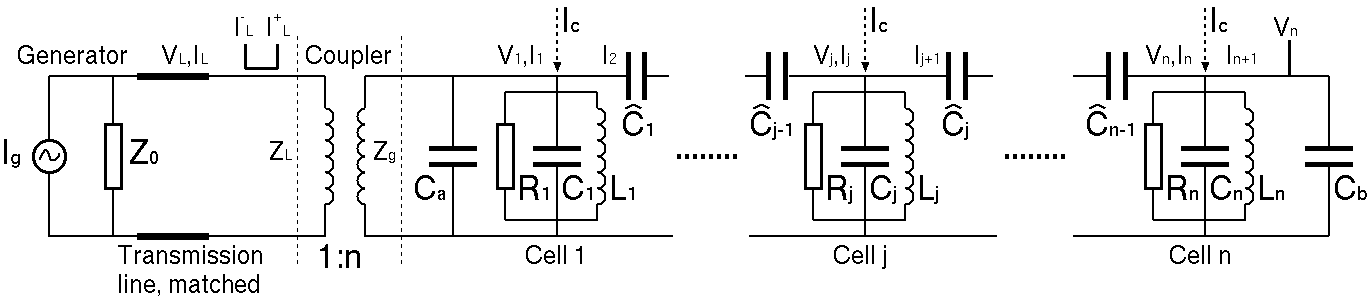
\includegraphics[width=0.99\textwidth]{./multicell2.png}
\end{center}
\caption{\label{fig:mcc}基于并联电路 RLC 谐振器的多单元腔，通过电容 $\hC$ 相互耦合，并由输入阻抗为 $Z_0$ 的发生器驱动。}
\end{figure}
% ..............................................
图~\ref{fig:mcc}给出了我们的模型。具有内阻 $Z_0$ 的发生器通过匹配传输线提供电流 $I_g$，并将其送入腔体。输入功率通过一个输入耦合器注入第一个单元，该耦合器用匝比为 $n$ 的变压器来建模。每个单元都表示为一个独立的 RLC 电路，相邻单元通过电容 $\hat C$ 耦合。此外，第一和最后一个单元还受到与束流管的耦合，这里用标记为 $C_a$ 和 $C_b$ 的电容来表示。我们还标出了穿过所有单元并在单元内部激发场的束流电流 $I_c$，不过在本文中我们不考虑这一效应，而只关注无束流情况下腔体的行为。特别是，我们考察单元间差异如何影响在耦合器上游紧邻处的定向耦合器测得的前向电流 $I^+_L$ 和反向电流 $I^-_L$，以及连接到最后一个单元、用于测量腔电压 $V_n$ 的场探针。耦合器两侧的参考平面用虚线表示。电压和电流与变压器匝比满足 $V_1=nV_L$ 和 $I_1=I_L/n$，因此阻抗 $Z_0=Z_L=V_L/I_L$ 与 $Z_g=V_1/I_1$ 之间有 $Z_g=n^2Z_L$ 的关系。
\par
在处理完整的时变问题之前，我们先简要讨论裸多单元腔的稳态。该分析遵循~\cite{PKH}中的讨论，并帮助我们确定束流管电容 $C_a$ 和 $C_b$ 的取值，以及腔体中支持的本征频率和相应本征模。与~\cite{PKH,LIEPE}中基于串联谐振电路的讨论不同，我们这里采用并联电路。
%
\section{稳态}
\label{sec:ss}
%
%..............................................
\begin{figure}[tb]
\begin{center}
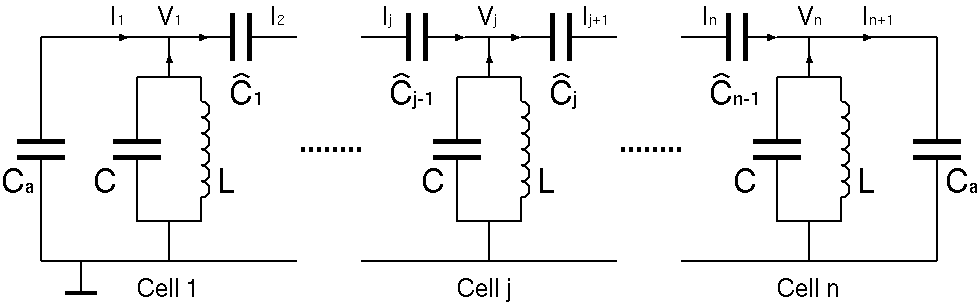
\includegraphics[width=0.8\textwidth]{./multicell_bare.png}
\end{center}
\caption{\label{fig:mcb}未加驱动的多单元腔，去掉了与发生器和电阻的耦合。不过，请注意表示与束流管耦合的电容 $C_a$ 和 $C_b$。}
\end{figure}
% ..............................................
为了确定 $C_a$ 和 $C_b$，我们分析图~\ref{fig:mcb}所示的简化模型，其中去掉了发生器和耦合器。此外，所有腔单元之间的电容都假定相等，并且由于简化模型的前后对称性，取 $C_a=C_b$。我们添加了接地符号，用以表示电压测量的参考电位。
\par
我们假设系统以频率 $\omega$ 振荡，因此可以用阻抗 $Z_C=1/i\omega C$ 和 $Z_L=i\omega L$ 分别表征电容和电感。于是，对电压为 $V_1$ 的第一个节点进行电流平衡，可得
\begin{equation}
  0=I_1-I_2+I_{LC}
  =i\omega C_a V_1 -i\omega \hC (V_2-V_1) + \left(i\omega C+\frac{1}{i\omega L}\right) V_1\ ,
\end{equation}
这里 $I_{LC}$ 是从地流向标记为 $V_1$ 的节点的电流。将该方程除以 $i\omega C$，并引入缩写 $\kappa_a=C_a/C$ 和 $\ho^2=1/LC$，我们得到
\begin{equation}\label{eq:c1}
  \left(1+\kappa+\kappa_a\right)V_1-\kappa V_2 = \frac{\ho^2}{\omega^2}V_1\ .
\end{equation}
同样地，第 $j$ 个单元的电流平衡给出
\begin{equation}
  0=I_j-I_{j-1}+I_{LC}
  = i\omega\hC(V_j-V_{j-1}) - i\omega\hC(V_{j+1}-V_j) + \left(i\omega C+\frac{1}{i\omega L}\right) V_j\ .
\end{equation}
再除以 $i\omega C$ 并稍作整理后得到
\begin{equation}\label{eq:cj}
  -\kappa V_{j-1}+(1+2\kappa)V_j-\kappa V_{j+1} =\frac{\ho^2}{\omega^2}V_j\ .
\end{equation}
对最右端标记为 $V_n$ 的节点重复上述分析，最终得到
\begin{equation}
0=i\omega\hC(V_n-V_{n-1})+ \left(i\omega C+\frac{1}{i\omega L}\right) V_j - i\omega C_a (0-V_n)
\end{equation}
并在引入缩写后得到
\begin{equation}\label{eq:cn}
  -\kappa V_{n-1}+(1+\kappa+\kappa_a)V_n= \frac{\ho^2}{\omega^2}V_n\ .
\end{equation}
综合起来，方程~\ref{eq:c1}、\ref{eq:cj} 和~\ref{eq:cn} 可以写成下面的本征值方程
\begin{equation}\label{eq:evs}
  \left(
    \begin{array}{ccccc}
      1+\kappa+\kappa_a & -\kappa & 0 & 0 & 0 \\
      -\kappa & 1+ 2\kappa & -\kappa & 0 & 0 \\
      0  &-\kappa & 1+ 2\kappa & -\kappa &  \\
      0 &0  &-\kappa & 1+ 2\kappa & -\kappa \\
      0  & 0  & 0  & -\kappa & 1+\kappa+\kappa_a
    \end{array}
  \right)
  \left(\begin{array}{c} V_1\\ V_2\\ V_3\\ V_4\\ V_5\end{array}\right)
  = \frac{\ho^2}{\omega^2}
  \left(\begin{array}{c} V_1\\ V_2\\ V_3\\ V_4\\ V_5\end{array}\right)
\end{equation}
这里我们假设 $n=5$。推广到其他单元数 $n$ 是很直接的。
\par
我们沿用~\cite{PKH}的做法，要求 $\pi$ 模在相邻单元中产生交替符号的电压：$(V_1,V_2,V_3,\dots)=(1,-1,1,\dots)$。将这一要求施加到方程~\ref{eq:evs}上，并考察前两行，可得条件
\begin{equation}
  1+2\kappa+\kappa_a  = \frac{\ho^2}{\opi^2}
  \qquad\mathrm{and}\qquad
  -1-4\kappa = -\frac{\ho^2}{\opi^2}\ .
\end{equation}
解出 $\kappa_a$ 和 $\ho^2/\opi^2$ 得到
\begin{equation}\label{eq:sol}
  \kappa_a=2\kappa
  \qquad\mathrm{and}\qquad
  \opi = \frac{\ho}{\sqrt{1+4\kappa}}\ .
\end{equation}
我们需要指出，在我们的模型中，$\pi$ 模频率位于单元谐振频率 $\ho$ 之下，这是采用并联谐振电路所产生的人为结果。在串联谐振电路中，$\pi$ 模频率则高于 $\ho$。
\par
既然已经知道 $\kappa_a$ 应取何值，我们将其代入方程~\ref{eq:evs}，得到下面这个已经正确匹配的本征值方程
\begin{equation}\label{eq:evs2}
  \left(
    \begin{array}{ccccc}
      1+3\kappa & -\kappa & 0 & 0 & 0 \\
      -\kappa & 1+ 2\kappa & -\kappa & 0 & 0 \\
      0  &-\kappa & 1+ 2\kappa & -\kappa &  \\
      0 &0  &-\kappa & 1+ 2\kappa & -\kappa \\
      0  & 0  & 0  & -\kappa & 1+3\kappa
    \end{array}
  \right)
  \left(\begin{array}{c} V_1\\ V_2\\ V_3\\ V_4\\ V_5\end{array}\right)
  = \frac{\ho^2}{\omega^2}
  \left(\begin{array}{c} V_1\\ V_2\\ V_3\\ V_4\\ V_5\end{array}\right)
\end{equation}
我们将进一步考察它，以确定所有本征频率和本征模。正如前面提到的，~\cite{PKH}中的相应方程是从串联电路模型推导出来的，而这里采用的是并联电路模型。因此，尽管方程~\ref{eq:evs2}的结构与~\cite{PKH}中的相应方程相似，但常数的定义不同，因此无法一一对应。
%..............................................
\begin{figure}[tb]
\begin{center}
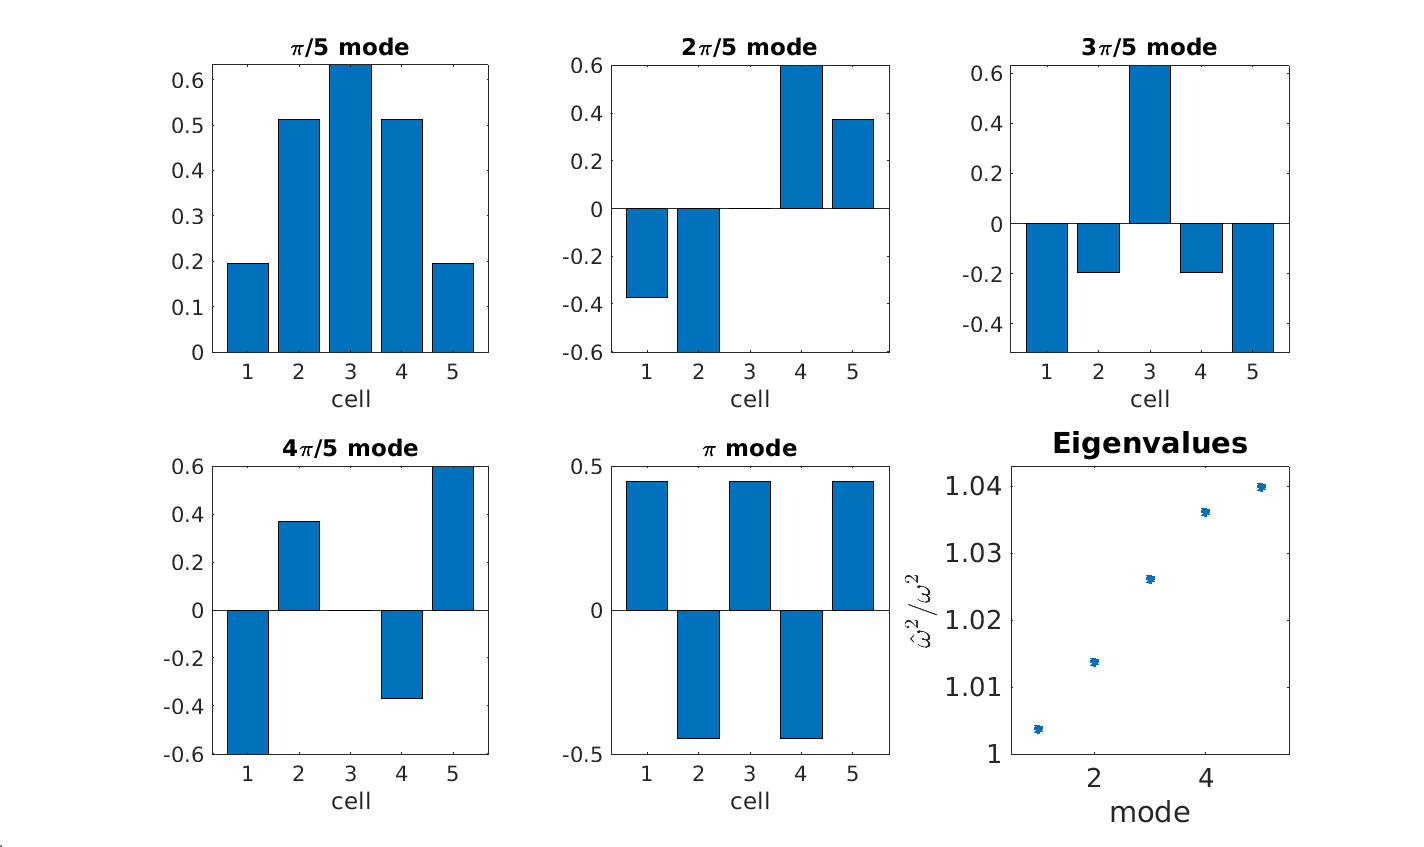
\includegraphics[width=0.9\textwidth]{./five_cell_modes.png}
\end{center}
\caption{\label{fig:evs}$\kappa=0.01$ 时五单元腔的模态与本征值。}
\end{figure}
% ..............................................
\par
实际上，方程~\ref{eq:evs2}中矩阵具有很高的对称性，因此其本征值和本征矢可以解析表示，~\cite{PKH}中就采用了这种方法，但我们这里不重复这些结果。相反，我们使用 Matlab 对相应量进行数值计算。图~\ref{fig:evs}在标为 $n\pi/5$ 模的图中给出了 $\kappa=0.01$ 时的五个本征模，并在右下角图中给出了相应的本征值。这里模式~1 对应 $\pi/5$ 模，模式~2 对应 $2\pi/5$ 模。特别地，我们看到，模式~5 的最大本征值对应于 $\pi$ 模，其数值为 $\hat\omega^2/\opi^2=1.04$，与方程~\ref{eq:sol}一致。
\par
如果我们用各自的频率激发不同的模式，组合后的激励分布就可以被塑造成在不同单元中达到峰值。腔体等离子体处理~\cite{PLASMA}正是利用了这一特性。它使我们能够在某个特定单元中局部激发等离子体，以对其进行清洗。
\par
%..............................................
\begin{figure}[tb]
\begin{center}
  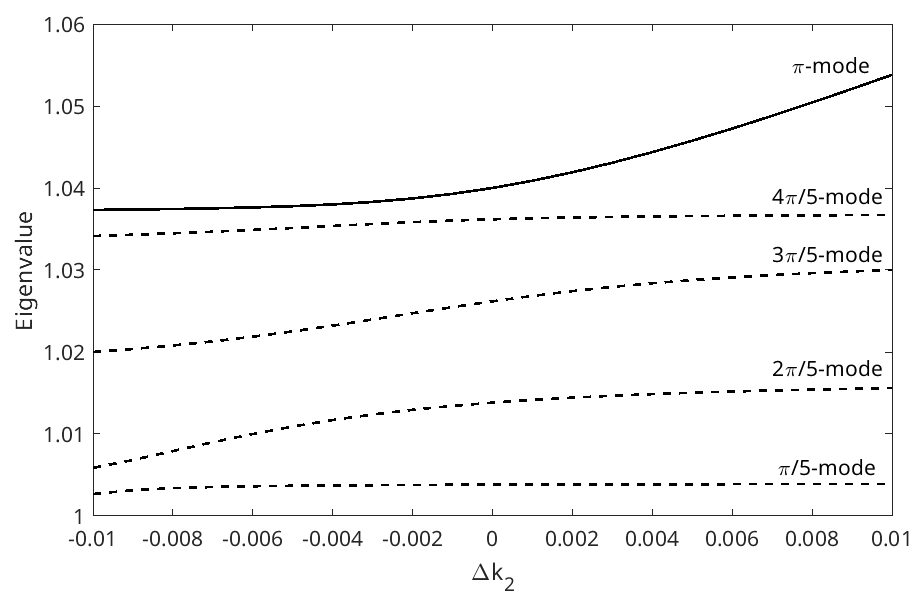
\includegraphics[width=0.47\textwidth]{./10-eigenvalues-vs-delta-kappa2.png}
  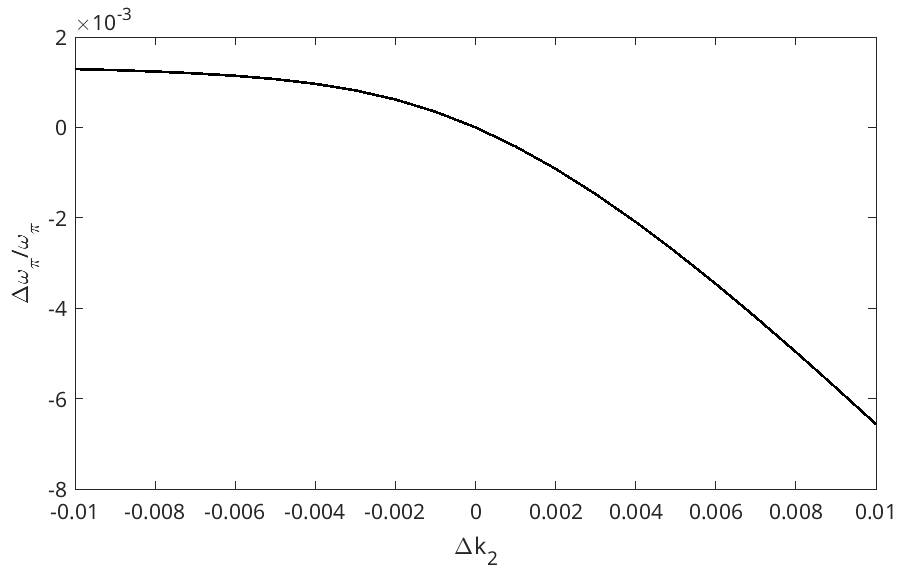
\includegraphics[width=0.49\textwidth]{./10-frequency-of-pi-mode-vs-delta-kappa2.png}
\end{center}
\caption{\label{fig:dk2}本征值随误差 $\Dk_2$ 的变化（左），以及 $\pi$ 模的相对频率偏移 $\Delta\omega_{\pi}/\omega_{\pi}$（右）。}
\end{figure}
% ..............................................
研究某个单元中耦合 $\kappa$ 的误差对本征频率的敏感性是很有启发性的。图~\ref{fig:dk2}右图显示的是第二与第三个单元之间的耦合 $\kappa_2$ 变化时的本征值。这里选择的范围相当大：$\Dk_2=-0.01$ 对应于耦合消失，而 $\Dk_2=0.01$ 对应于设计值加倍。我们观察到，尤其是 $\pi$ 模的本征值会显著增大，特别是在 $\Dk_2$ 为正时更为明显。右图显示了由本征值推导得到的相对频率变化 $\Delta\omega_{\pi}/\omega_{\pi}$，在所选范围内它几乎变化了百分之一。曲线在 $\Dk_2=0$ 附近的斜率给出了本征频率对 $\Dk_2$ 的敏感度。对更小范围内扫描 $\Dk_2$ 所做的拟合表明
\begin{equation}
  \Delta\left(\Delta\omega_{\pi}/\omega_{\pi}\right)=-0.38\,\Dk_2\ ,
\end{equation}
考虑到超导腔极窄的带宽，这个数值已经很大。因此，$\Dk_2=10^{-4}$ 的误差就会把频率移出腔体带宽。
\par
本节的分析纯属静态。不过在后续各节中，我们会把它扩展到瞬态现象。在这个过程中，我们还会给单个单元引入特定缺陷，从而研究它们的后果。
%
\section{模型}
\label{sec:mod}
%
现在考虑腔体中部第~$j$ 个单元的 $RLC$ 支路中流过的电流 $I_j$。第一和最后一个单元需要特殊处理，我们稍后再回到它们。标记为 $V_j$ 的节点处的电流平衡由分别流经 $R$、$L$ 和 $C$ 的电流之和给出。因此我们得到~\cite{VZAP}
\begin{equation}\label{eq:RLC}
  0=I_j-I_{j+1}+\frac{V_j}{R_j}+\frac{1}{L_j}\int V_j dt+ C_j\frac{dV_j}{dt}
\end{equation}
电流 $I_j$ 和 $I_{j+1}$ 分别通过电容 $\hat C_{j-1}$ 和 $\hat C_j$，并由相邻单元中电压 $V_j$ 的差值决定
\begin{equation}
  I_j=\hC_{j-1}\left[\frac{dV_j}{dt}-\frac{dV_{j-1}}{dt}\right]
  \qquad\mathrm{and}\qquad
  I_{j+1}=\hC_{j}\left[\frac{dV_{j+1}}{dt}-\frac{dV_{j}}{dt}\right] \ . 
\end{equation}
将其代入方程~\ref{eq:RLC}后得到
\begin{equation}
  0=-\hC_{j-1}\frac{dV_{j-1}}{dt} -\hC_{j+1}\frac{dV_{j+1}}{dt} + \frac{V_j}{R_j}
  +\frac{1}{L_j}\int V_j dt+ \left(C_j+\hC_{j-1}+\hC_{j+1}\right)\frac{dV_j}{dt}\ .
\end{equation}
将其除以 $C_j$，并引入缩写 $\kappa'_j=\hC_{j-1}/C_j$ 和 $\kappa_j=\hC_{j+1}/C_j$，该方程变为
\begin{eqnarray}\label{eq:cellj}
  0&=&-\kappa'_j\frac{dV_{j-1}}{dt}-\kappa_j\frac{dV_{j+1}}{dt}+ \frac{V_j}{R_jC_j}
       +\frac{1}{L_jC_j}\int V_j dt+ \left(1+\kappa'_j+\kappa_j\right)\frac{dV_j}{dt}
  \nonumber\\
   &=&-\kappa'_j\frac{dV_{j-1}}{dt}-\kappa_j\frac{dV_{j+1}}{dt}+ \frac{\ho_j}{Q_j}V_j
       +\ho_j^2\int V_j dt+ \left(1+\kappa'_j+\kappa_j\right)\frac{dV_j}{dt}\ ,
\end{eqnarray}
这里在第二个等号中使用了缩写 $1/L_jC_j=\ho_j^2$ 和 $R_jC_j=Q_j/\ho_j$。此时我们引入 $V_j=\tV_je^{i\omega t}$ 的慢变幅度 $\tV_j$，于是可以写成~\cite{VZAP}
\begin{equation}\label{eq:harm}
  \frac{dV_j}{dt}=e^{i\omega t}\left[i\omega\tV_j + \frac{d\tV_j}{dt}\right]
  \qquad\mathrm{and}\qquad
  \int V_j dt = \frac{e^{i\omega t}}{\omega^2}\left[-i\omega\tV_j + \frac{d\tV_j}{dt}\right]\ ,
\end{equation}
其中 $j=1,\dots,n$。这里我们忽略二阶导数 $d^2\tV_j/dt^2$，而 $\omega$ 是发生器工作的频率。将其代入方程~\ref{eq:cellj}，消去公共指数因子 $e^{i\omega t}$ 并稍作整理后，得到
\begin{eqnarray}\label{eq:tmp1}
  0&=&-\kappa'_j \frac{d\tV_{j-1}}{dt}-\kappa_j \frac{d\tV_{j+1}}{dt}
  +\left(1+\kappa'_j+\kappa_j+\frac{\ho_j^2}{\omega^2}\right)\frac{d\tV_j}{dt} \\
   &&\quad + \frac{\ho_j}{Q_j}\tV_j+i\omega\left[-\kappa'_j\tV_{j-1}-\kappa_j\tV_{j+1} 
      +\left(1+\kappa'_j+\kappa_j-\frac{\ho_j^2}{\omega^2}\right)\tV_j\right]\ .\nonumber
\end{eqnarray}
只要所有 $\kappa'_j$ 和 $\kappa_j$ 都相等，方括号中的量就等价于方程~\ref{eq:cj}。使该括号为零的 $\omega$ 值因此决定了方程~\ref{eq:evs}中矩阵的本征值，而这些本征值描述了系统的稳态，因为在这种情况下，电压对时间的导数也必须为零。与 $\ho_j/Q_j$ 成正比的附加项来自有限电阻 $R_j$，描述的是阻尼。这一项在第~\ref{sec:ss}节的讨论中并不存在。为了便于后文引用，我们将方程~\ref{eq:tmp1}改写为
\begin{eqnarray}\label{eq:cjt}
  &&-\kappa'_j \frac{d\tV_{j-1}}{dt}
     +\left(1+\kappa'_j+\kappa_j+\frac{\ho_j^2}{\omega^2}\right)\frac{d\tV_j}{dt}
  -\kappa_j \frac{d\tV_{j+1}}{dt}\\
   &&\quad = -\frac{\ho_j}{Q_j}\tV_j-i\omega\left[-\kappa'_j\tV_{j-1}
      +\left(1+\kappa'_j+\kappa_j-\frac{\ho_j^2}{\omega^2}\right)\tV_j-\kappa_j\tV_{j+1} \right]\ ,\nonumber
\end{eqnarray}
这样就把含导数的项放在等式左边，其余项放在右边。
\par
对于最后一个单元~$n$，我们从图~\ref{fig:mcc}中标记为 $V_n$ 的节点上的电流平衡出发
\begin{equation}
  0=I_n-I_{n+1}+\frac{V_n}{R_n} +\frac{1}{L_n}\int V_ndt + C_n\frac{dV_n}{dt}
\end{equation}
并将电流表示为相邻节点电压的函数
\begin{equation}
  I_n=\hC_{n-1}\left[\frac{dV_j}{dt}-\frac{dV_{j-1}}{dt}\right]
  \qquad\mathrm{and}\qquad
  I_{n+1}=C_b\left[0-\frac{dV_{n}}{dt}\right] \ , 
\end{equation}
其中电容 $C_b$ 的另一端接地，这就解释了方括号中的零。整理各项并引入缩写 $\kappa'_n=\hC_{n-1}/C_n$ 和 $\kappa_b=C_b/C_n$ 后得到
\begin{equation}
  0=-\kappa'_n \frac{dV_{n-1}}{dt}+\left(1+\kappa'_n+\kappa_b\right)  \frac{dV_{n}}{dt} 
  + \frac{\ho_n}{Q_n}V_n +\ho_n^2\int V_n dt\ , 
\end{equation}
其中我们引入了 $1/L_nC_n=\ho_n^2$ 和 $R_nC_n=Q_n/\ho_n$。借助方程~\ref{eq:harm}，并在消去公共指数因子 $e^{i\omega t}$ 后，该方程变为
\begin{eqnarray}
  0&=&-\kappa'_n \frac{d\tV_{n-1}}{dt}
  +\left(1+\kappa'_n+\kappa_b+\frac{\ho_n^2}{\omega^2}\right)\frac{d\tV_j}{dt} \\
   &&\quad + \frac{\ho_n}{Q_n}\tV_n+i\omega\left[-\kappa'_n\tV_{n-1}
      +\left(1+\kappa'_n+\kappa_b-\frac{\ho_n^2}{\omega^2}\right)\tV_n\right]\ .\nonumber
\end{eqnarray}
与前面一样，方括号中的量对应方程~\ref{eq:cn}，并形成方程~\ref{eq:evs}矩阵的最后一行。稍作整理后得到
\begin{eqnarray}\label{eq:cnt}
  &&-\kappa'_n \frac{d\tV_{n-1}}{dt}
  +\left(1+\kappa'_n+\kappa_b+\frac{\ho_n^2}{\omega^2}\right)\frac{d\tV_j}{dt} \\
   &&\qquad = -\frac{\ho_n}{Q_n}\tV_n -i\omega\left[-\kappa'_n\tV_{n-1}
      +\left(1+\kappa'_n+\kappa_b-\frac{\ho_n^2}{\omega^2}\right)\tV_n\right]\ ,\nonumber
\end{eqnarray}
这里我们同样把导数项收集到等式左边。
\par
最后我们来看第一个单元，它还通过 $\hC_1$ 和 $C_a$ 上方的耦合器相连。该单元中标记为 $V_1$ 的节点处电流平衡为
\begin{eqnarray}
  \frac{I_g}{n} &=& \frac{V_1}{n^2Z_0} + \frac{V_1}{R_1}+\frac{1}{L_1}\int V_1dt
       + \left(C_1+C_a\right)\frac{dV_1}{dt} -I_2\\
   &=& \frac{I_g}{n}+\left( 1+\beta\right) \frac{V_1}{R_1} +\frac{1}{L_1}\int V_1dt
       + \left(C_1+C_a\right)\frac{dV_1}{dt} -\hC_1\left[\frac{dV_2}{dt}-\frac{dV_1}{dt}\right]\ ,
       \nonumber
\end{eqnarray}
这里引入耦合因子 $\beta=R_1/n^2Z_0$。需要注意的是，我们必须把阻抗 $Z_0$ 通过变压器变换到腔体内部，这解释了分母中的 $n^2$ 因子，以及在变压器“另一侧”将发生器电流 $I_g$ 除以 $n$。进一步将该方程除以 $C_1$，并引入缩写 $\kappa_1=\hC_1/C_1$ 和 $\kappa_a=C_a/C_1$ 后，我们得到
\begin{equation}
 \frac{1}{C_1}\frac{I_g}{n} =(1+\beta)\frac{\ho_1}{Q_1}V_1
  +\ho_1^2\int V_1dt+\left(1+\kappa_a+\kappa_1\right)\frac{dV_1}{dt} -\kappa_1\frac{dV_2}{dt}\ .
\end{equation}
使用方程~\ref{eq:harm}并消去公共指数因子 $e^{i\omega t}$ 后，得到
\begin{eqnarray}\label{eq:c1ttemp}
  \frac{1}{C_1}\frac{\tilde I_g}{n}&=&\left(1+\kappa_a+\kappa_1+\frac{\ho_1^2}{\omega^2}\right)\frac{d\tV_1}{dt}
       -\kappa_1\frac{d\tV_2}{dt}\\
     &&\qquad  +(1+\beta)\frac{\ho_1}{Q_1}\tV_1
        +i\omega\left[\left(1+\kappa_a+\kappa_1-\frac{\ho_1^2}{\omega^2}\right)\tV_1
        -\kappa_1\tV_2\right]\ .\nonumber
\end{eqnarray}
方括号中的量描述了方程~\ref{eq:c1}，并对应于方程~\ref{eq:evs}矩阵的第一行。现在我们引入加载 $Q$ 值 $Q'_L=Q_1/(1+\beta)$，并注意到 $1/C_1=\ho_1R_1/Q_1=\ho_1R_1/(1+\beta)Q'_L$。这里 $Q'_L$ 只是第一个单元的加载 $Q$ 值。顺便指出，文献中经常出现的写法是 $(1+\beta)Q'_L$，而不是 $Q_1$。重新整理方程~\ref{eq:c1ttemp} 后，我们得到
\begin{eqnarray}\label{eq:c1t}
  &&\left(1+\kappa_a+\kappa_1+\frac{\ho_1^2}{\omega^2}\right)\frac{d\tV_1}{dt}
  -\kappa_1\frac{d\tV_2}{dt}\\
     &&\qquad=-\frac{\ho_1}{Q'_L}\tV_1
        -i\omega\left[\left(1+\kappa_a+\kappa_1-\frac{\ho_1^2}{\omega^2}\right)\tV_1
        -\kappa_1\tV_2\right] + \frac{\ho_1R_1}{Q_1}\frac{\tilde I_g}{n}\ .\nonumber
\end{eqnarray}
在没有耦合的情况下，我们只需处理一个单元和一个频率约为 $\omega\approx\ho_1$ 的模态。此时，该方程化简为 $2d\tV_1/dt=-(\ho_1/Q'_L)\tV_1-i\ho_1\delta_1\tV_1+\ho_1R_1/((1+\beta)Q'_L){\tilde I_g}/n$，其中失谐量 $\delta_1=\omega/\ho_1-\ho_1/\omega$，这与~\cite{VZAP}中单个谐振器的计算一致。
\par
方程~\ref{eq:cjt}、\ref{eq:cnt} 和~\ref{eq:c1t} 描述了在发生器以频率~$\omega$ 激励时多单元腔的动力学行为。在接下来的章节中，我们将考虑最重要的情形，即腔体被驱动到激发 $\pi$ 模。
% 
\section{完美 $\pi$-模腔}
%
这里我们假设发生器工作的频率为 $\opi=\ho/\sqrt{1+4\kappa}$，其中 $\ho$ 是单个单元谐振频率的设计值，$\kappa$ 是相邻单元之间耦合的设计值。$Q$ 是各单元的本征品质因数，并且都假定相同。对于设计值 $\kappa_a=\kappa_b=2\kappa$，我们可以把描述第一个单元的方程~\ref{eq:c1t}化为
\begin{eqnarray}\label{eq:c1tp}
\left(2+7\kappa\right)\frac{d\tV_1}{dt} -\kappa\frac{d\tV_2}{dt}
     &=&-\frac{\ho}{Q'_L}\tV_1
        -i\opi\left[-\kappa\tV_1
         -\kappa\tV_2\right] + \frac{\ho R_1}{Q_1}\frac{\tilde I_g}{n}\\
     &=&-\frac{\ho}{Q'_L}\tV_1
         +i\frac{\ho\kappa}{\sqrt{1+4\kappa}}\left[\tV_1+\tV_2\right]
         + \frac{\ho R_1}{Q_1}\frac{\tilde I_g}{n}\ .\nonumber
\end{eqnarray}
其中 $Q'_L=Q/(1+\beta)$。同样，位于腔体中部、满足 $2\leq j \leq n-1$ 的第 $j$ 个单元的方程基于方程~\ref{eq:cjt}，并化为
\begin{eqnarray}\label{eq:cjtp}
&&  -\kappa \frac{d\tV_{j-1}}{dt} +\left(2+6\kappa\right)\frac{d\tV_j}{dt}
     -\kappa \frac{d\tV_{j+1}}{dt}\nonumber\\
   &&\qquad\qquad= -\frac{\ho}{Q}\tV_j-i\opi\left[-\kappa\tV_{j-1}
      -2\kappa\tV_j-\kappa\tV_{j+1} \right] \\
  &&\qquad\qquad = -\frac{\ho}{Q}\tV_j+i\frac{\ho\kappa}{\sqrt{1+4\kappa}}
     \left[\tV_{j-1} +2\tV_j+\tV_{j+1} \right]\ .\nonumber
\end{eqnarray}
最后，对于第 $n$ 个单元，我们利用方程~\ref{eq:cnt}，它变为
\begin{eqnarray}\label{eq:cntp}
  -\kappa \frac{d\tV_{n-1}}{dt}+\left(2+7\kappa\right)\frac{d\tV_j}{dt} 
  &=& -\frac{\ho}{Q}\tV_n -i\opi\left[-\kappa\tV_{n-1}-\kappa\tV_n\right]\\
  &=& -\frac{\ho}{Q}\tV_n +i\frac{\ho\kappa}{\sqrt{1+4\kappa}}
      \left[\tV_{n-1}+\tV_n\right]\nonumber
\end{eqnarray}
因此，这三个方程描述了一个在 $\pi$ 模下工作的完美多单元腔的瞬态行为。
\par
在仿真中，我们将方程乘以 $\dt$，这样数值上更稳定，因为此时大多数因子的量级都接近 1。进一步地，我们将方程~\ref{eq:c1tp}、\ref{eq:cjtp} 和~\ref{eq:cntp}变换成下面的矩阵方程
\begin{equation}\label{eq:dynp}
%  D\frac{d\vec V}{dt}\dt = -(A-iB)\vec V +\frac{\ho\dt R_1}{(1+\beta)Q'_L}\vec I
  D\frac{d\vec V}{dt}\dt = -(A-iB)\vec V +\frac{\ho\dt R_1}{Q_1}\vec I
\end{equation}
其中我们使用了如下缩写
\begin{eqnarray}\label{eq:dynpaux}
  \vec V &=& \left(\tV_1,\tV_2,\tV_3,\tV_4,\tV_5\right)^{\top}\nonumber\\
  \frac{d\vec V}{dt} &=&
       \left(\frac{d\tV_1}{dt} , \frac{d\tV_2}{dt} , \frac{d\tV_3}{dt} , 
       \frac{d\tV_4}{dt} , \frac{d\tV_5}{dt} \right)^{\top}\nonumber\\
  \vec I &=& \left(\tilde I_g/n,0,0,0,0\right)^{\top}\nonumber\\
  D&=&\left(\begin{array}{ccccc}
     2+7\kappa & -\kappa & 0 & 0 & 0 \\
     -\kappa & 2+6\kappa & - \kappa & 0 & 0 \\
     0 & -\kappa & 2+6\kappa & - \kappa & 0 \\
     0 & 0 & -\kappa & 2+6\kappa & - \kappa \\
     0 & 0 &  0 &-\kappa & 2+7\kappa
   \end{array}\right)\\
  A&=&\diag\left((1+\beta)\frac{\ho\dt}{Q}, \frac{\ho\dt}{Q}, \frac{\ho\dt}{Q},
       \frac{\ho\dt}{Q}, \frac{\ho\dt}{Q}\right)\nonumber\\
  B&=&\frac{\ho\dt\kappa}{\sqrt{1+4\kappa}}\left(\begin{array}{ccccc}
              1 & 1 & 0 & 0 & 0\\
              1 & 2 & 1 & 0 & 0\\
              0 & 1 & 2 & 1 & 0\\
              0 & 0 & 1 & 2 & 1\\
              0 & 0 & 0 & 1 & 1
 \end{array}\right)\ . \nonumber
\end{eqnarray}
我们进一步通过引入电压和电流的实部与虚部来改写系统
\begin{equation}
  \vec V = \vec V_r + i\vec V_i
  \qquad\mathrm{and}\qquad
  \vec I = \vec I_r + i\vec I_i \ . 
\end{equation}
这把方程~\ref{eq:dynp}变换为
\begin{equation}\label{eq:dynpb}
  \left(\begin{array}{cc} D & 0_5 \\ 0_5 & D\end{array}\right)
  \left(\begin{array}{c} \frac{d\vec V_r}{dt} \\ \frac{d\vec V_i}{dt}\end{array}\right)\dt
  =-\left(\begin{array}{rr} A & B \\ -B & A\end{array}\right)
  \left(\begin{array}{c} \vec V_r \\ \vec V_i\end{array}\right)
  +\frac{\ho\dt R_1}{Q_1} \left(\begin{array}{c} \vec I_r \\ \vec I_i\end{array}\right)\ ,
\end{equation}
其中 $0_5$ 是一个仅含零元素的 $5\times 5$ 矩阵。此时我们处理的是五个单元电压的 10 个实部与虚部，等价地说，就是 I 和 Q 分量。
\par
稳态条件对应于左边时间导数为零，这就给出了稳态电压
\begin{equation}
  \tilde V_{\infty} =
  \left(\begin{array}{c} \vec V_r \\ \vec V_i\end{array}\right)_{\infty}
  = \frac{\ho\dt R_1}{Q_1}
  \left(\begin{array}{rr} A & B \\ -B & A\end{array}\right)^{-1}
  \left(\begin{array}{c} \vec I_r \\ \vec I_i\end{array}\right)\ .
\end{equation}
其中我们引入 $\tilde V=(\vec V_r,\vec V_i)^{\top}$。
\par
由方程~\ref{eq:dynpb}可得电压 $\tilde V$ 随重标度时间 $s=t/\dt$ 的演化
\begin{equation}\label{eq:dynpc}
  \frac{d\tilde V}{ds} = -\tilde A \tilde V(s)+\frac{\ho\dt R_1}{Q_1}\tilde I
  \quad\mathrm{with}\quad
  \tilde A=\left(\begin{array}{rr} D^{-1}A & D^{-1}B \\ -D^{-1}B & D^{-1}A\end{array}\right)
\end{equation}
以及 $\tilde I(s)=(D^{-1}I_r, D^{-1}I_i)^{\top}$。注意这里 $\tilde V$ 和 $\tilde I$ 都依赖于 $s$。
\par
在这里，$\tilde A$ 和 $\tilde I$ 都是常数，因此我们可以对方程~\ref{eq:dynpc}形式积分，得到
\begin{equation}
  \tilde V(s)=\exp\left[-\tilde A s\right]\tilde K + \tilde V_{\infty}\ ,
\end{equation}
其中 $\tilde K$ 是包含电压积分常数的向量。匹配初始条件 $\tilde V(s=0)=\tilde V_0$ 后，有 $\tilde K=\tilde V_0-\tilde V_{\infty}$，从而得到形式解
\begin{equation}\label{eq:dynpd}
  \tilde V(s)=\exp\left[-\tilde A s\right]\left(\tilde V_0-\tilde V_{\infty}\right)
  + \tilde V_{\infty}\ ,
\end{equation}
其中不同的 $\tilde V$ 都是 10 维向量，前五个分量为实部，下面五个分量为虚部。矩阵指数 $\exp\left[-\tilde A s\right]$ 是一个 $10\times 10$ 矩阵，可以由 $\tilde A$ 的本征分解计算得到。
\par
假设我们把 $\tilde A$ 通过其本征值和本征矢写成由 $W$ 组装的形式
\begin{equation}\label{eq:WLW}
  \tilde A= W\Lambda W^{-1}
  \qquad\mathrm{with}\qquad
  \Lambda=\diag\left(\lambda_1,\dots,\lambda_{10}\right)\ .
\end{equation}
现在设想把 $\exp\left[-\tilde A s\right]$ 展开成 $\tilde A s$ 的幂级数。此时很容易看出，计算 $\tilde A s$ 的幂总会把 $W$ 和 $W^{-1}$ 放到彼此相邻的位置，因此它们会相互抵消，只留下最前面和最后面的 $W$ 与 $W^{-1}$，中间则是 $(\Lambda s)$ 的幂。它们组合起来就构成矩阵指数
\begin{equation}\label{eq:expm}
  \exp\left[-\tilde A s\right]=W\left(e^{-\lambda_1s},\dots,e^{-\lambda_{10}s}\right) W^{-1}\ ,
\end{equation}
这就为我们提供了一个显式计算矩阵指数并数值求解方程~\ref{eq:dynpd}的方案。我们所需的只是 $\tilde A$ 的本征分解，而这可以轻松地用 Matlab 的内置函数 {\tt eig()} 完成。这种求电压的方法非常高效；我们只需调用一次 {\tt eig()}，然后对每个时刻 $s$，先计算方程~\ref{eq:expm}，再计算方程~\ref{eq:dynpd}。我们把该算法写成一个 Matlab 脚本，并运行 10000 个时间步，每步长度为 $\dt$。在仿真中，我们取耦合 $\beta=5000$、本征 $Q=10^9$、并联阻抗 $R=10^6\,\Omega$、谐振频率 $\ho/2\pi=1.5\,$GHz，以及单元间耦合 $\kappa=0.01$。此外，我们使用 $I_g/n=1\,$kA。
\par
%..............................................
\begin{figure}[tb]
\begin{center}
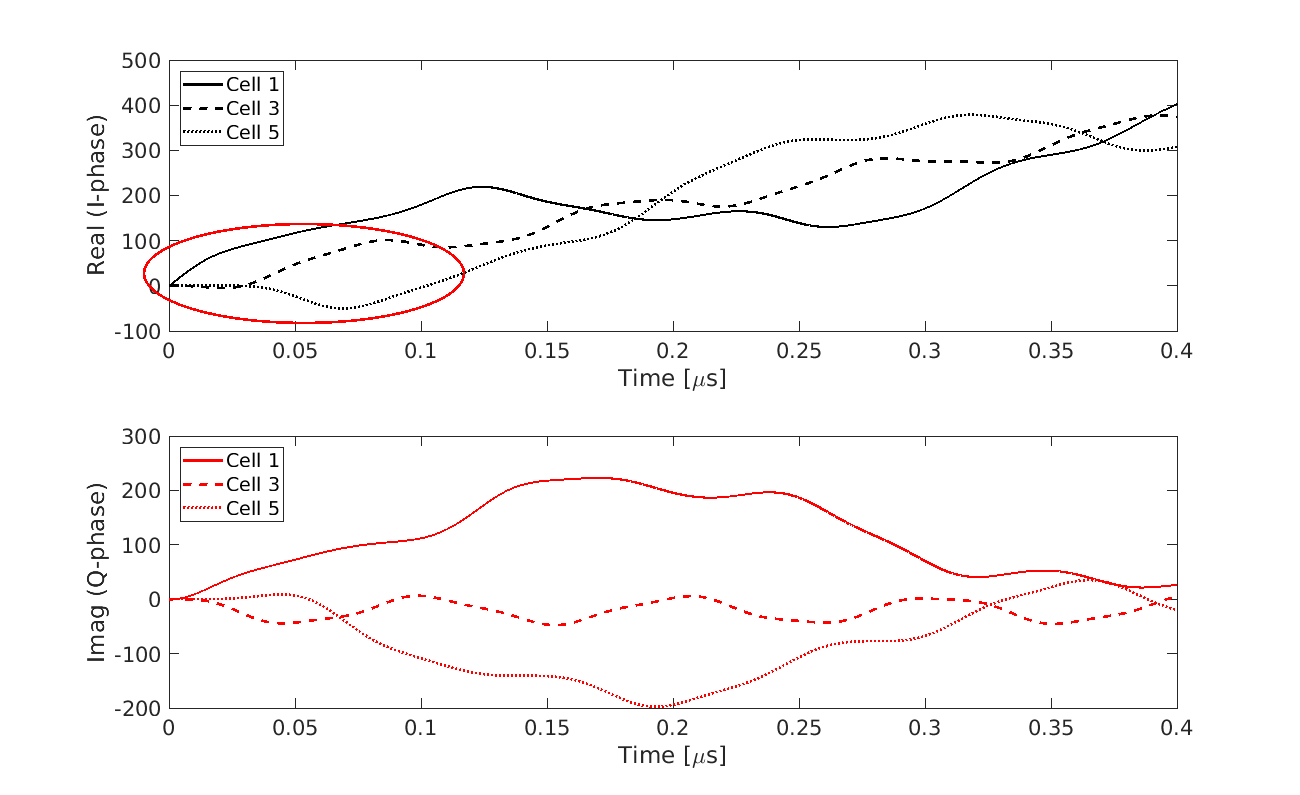
\includegraphics[width=0.49\textwidth]{./02-five-startup-04us.png}
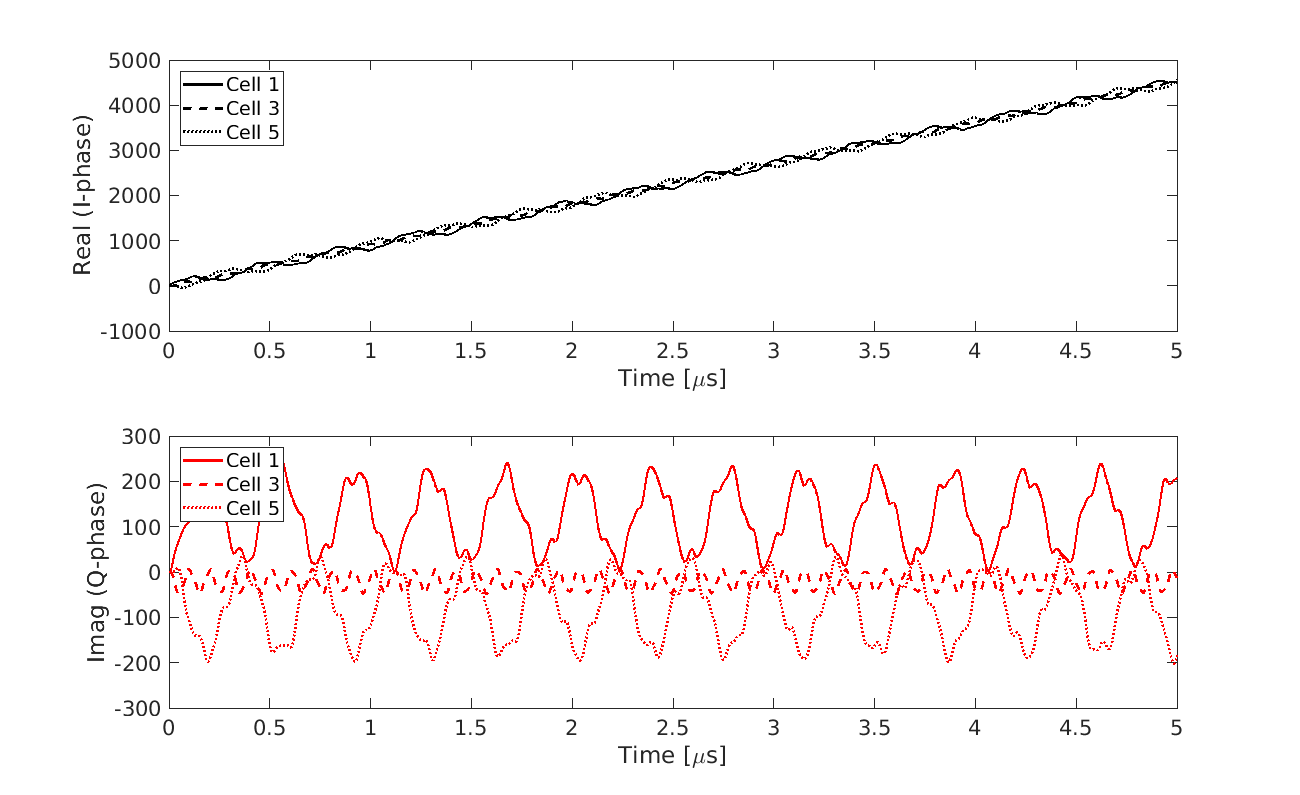
\includegraphics[width=0.49\textwidth]{./03-five-5us-IQ.png}
\end{center}
\caption{\label{fig:fivea}左图：发生器开启后的最初 0.4\,\textmu s 内，第 1、3、5 单元的实部（上）和虚部（下）。右图：前 5\,\textmu s 的对应信号。}
\end{figure}
% ..............................................
图~\ref{fig:fivea}左图上半部分显示第 1、3、5 单元电压的实部，下半部分显示对应的虚部。我们省略了第 2 和第 4 单元的场，因为它们与 $\pi$ 模中奇数单元的极性相反，画出来会让图过于复杂。该仿真中我们取 $\dt=4\times 10^{-11}\,$s，使横轴延伸到 0.4\,\textmu s。上图中我们用红色椭圆强调了启动过程：第 1 单元的场（实线）先上升，随后第 3 单元（虚线）上升，而稍后第 5 单元（点线）也开始上升。不过，在 0.2\,\textmu s 之后，场已经开始表现出整体增长。下图中的虚部只呈现来回拍振，没有整体增长。
\par
右图展示了把时间步长增大到 $\dt=5\times10^{-10}\,$s 的仿真，此时横轴延伸到 5\,\textmu s。现在，上图中三单元电场的实部明显呈线性上升，只有围绕线性上升的很小扰动。下图中的电压虚部也有一些拍振，但与上图相比幅度小得多。到这里我们已经可以得出结论：奇数单元中的场是同步上升的，这说明发生器实际上是把 $\pi$ 模作为一个整体来驱动，而不是先激发第 1 单元，再由它依次激发第 2 单元等等。单元之间的均衡发生在小于 1 微秒的时间尺度上。
\par
也许有人会想，图~\ref{fig:fivea}中看到的振荡能否被直接观测到，至少在透射信号上，也许在反射信号上也行。它们发生在 100\,ns 的时间尺度上，测量它们需要 10\,MHz 或更高的数据采集带宽。常规信号处理通常使用更小的带宽，因此这些振荡会被平均掉，可能不会被观察到。另一方面，为诊断目的进一步研究它们可能很有意思，我们以后会继续探索这一点。
\par
%..............................................
\begin{figure}[tb]
\begin{center}
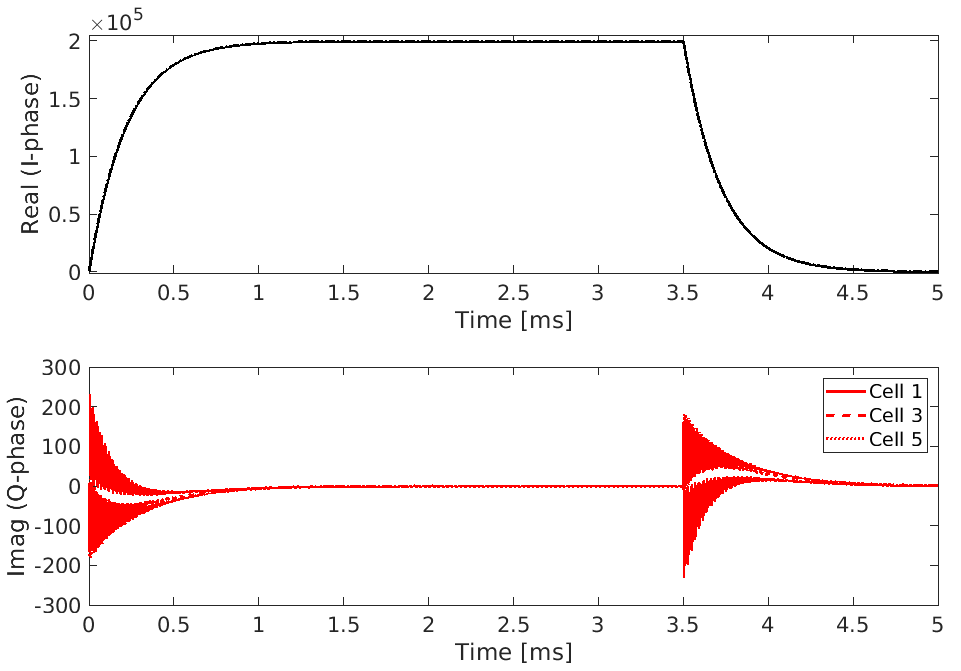
\includegraphics[width=0.9\textwidth]{./06-five-5ms-IQ-pulse.png}
\end{center}
\caption{\label{fig:fiveb}第 1、3、5 单元电压的实部（上）和虚部（下）。发生器在 0 到 3.5\,ms 之间开启。}
\end{figure}
% ..............................................
%..............................................
\begin{figure}[tb]
\begin{center}
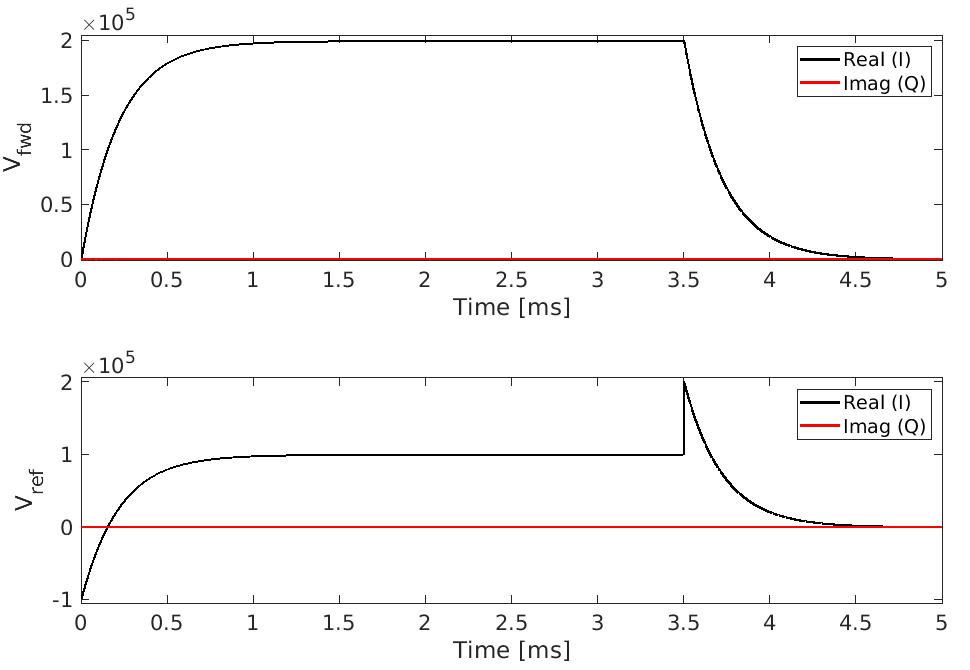
\includegraphics[width=0.9\textwidth]{./07-five-5ms-fwd-ref-pulse.png}
\end{center}
\caption{\label{fig:fivec}上图：假定由第 5 单元拾取的透射信号的实部和虚部。下图：反射信号的实部和虚部。发生器在 0 到 3.5\,ms 之间开启。}
\end{figure}
% ..............................................
图~\ref{fig:fiveb}显示的是一个 $\dt=5\times 10^{-7}\,$s 的仿真结果，因此横轴延伸到 5\,ms。除了在零时刻开启发生器，我们还在 3.5\,ms 后将其关闭。与前一样，电压的实部显示在上图。在这个时间尺度上，单元 1、3 和 5 的电压差异已经看不出来。它们表现出预期的行为：先给腔体充填，然后在 3.5\,ms 后发生器关闭时开始放电。我们注意到，在时刻零开启发生器之后以及 3.5\,ms 关闭发生器之后，下图中都会出现明显的扰动，不过其幅度远小于上图。
\par
图~\ref{fig:fivec}上图显示第 5 单元电压 $V_5$ 的实部和虚部，假定它装有一个场探针并提供透射信号。下图显示返回发生器方向的反射电压脉冲的实部和虚部。其表达式为~\cite{VZAP}
\begin{equation}
  nV_{ref}=V_1-\frac{R_1I_g/n}{2\beta}\ ,
\end{equation}
其中 $V_1$ 是第 1 单元的电压。该信号在脉冲开始时呈现明显的负尖峰，在脉冲结束时呈现正尖峰。
\par
%..............................................
\begin{figure}[p]
\begin{center}
  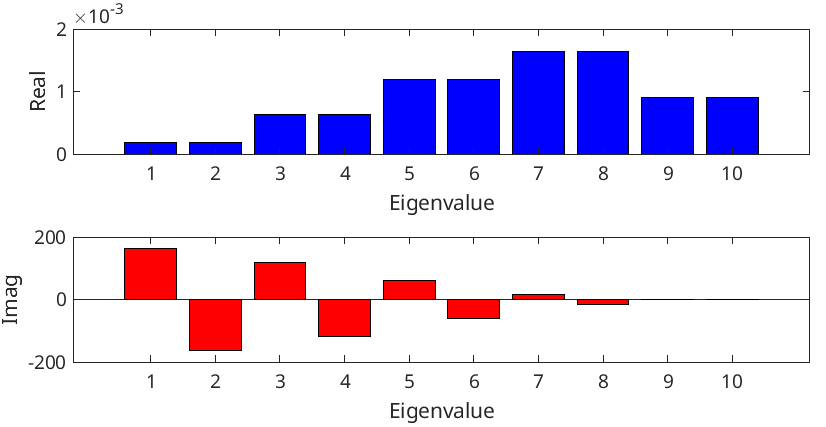
\includegraphics[width=0.65\textwidth]{./08-eigenvalues.png}
  \caption{\label{fig:eigval}$\tilde A$ 本征值的实部（上）和虚部（下）。}
  \vskip 5mm
  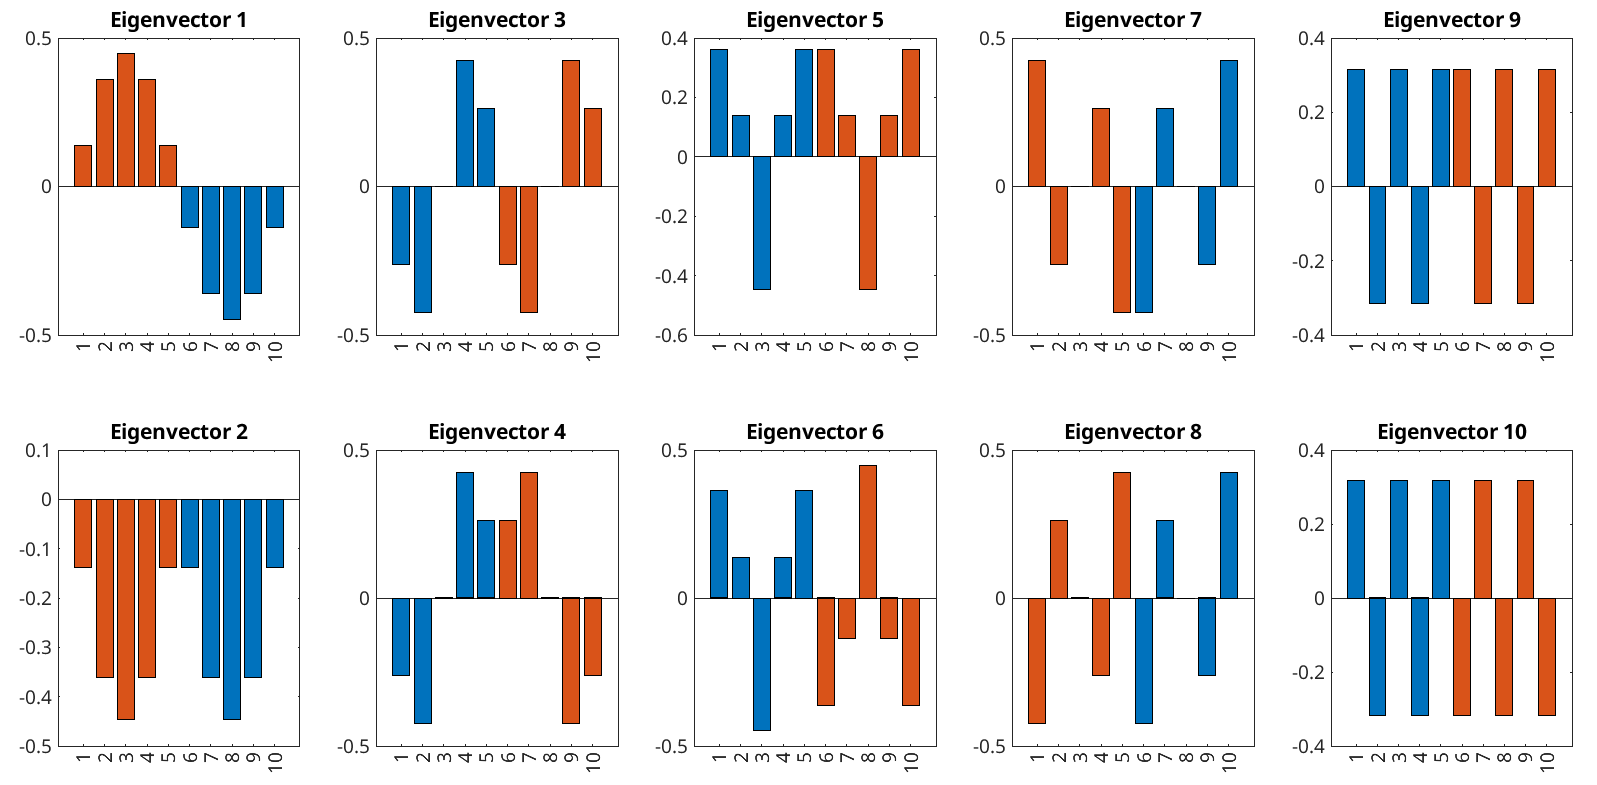
\includegraphics[width=0.65\textwidth]{./08-eigenvectors.png}
  \caption{\label{fig:eigvec}$\tilde A$ 的本征矢。}
  \vskip 5mm
  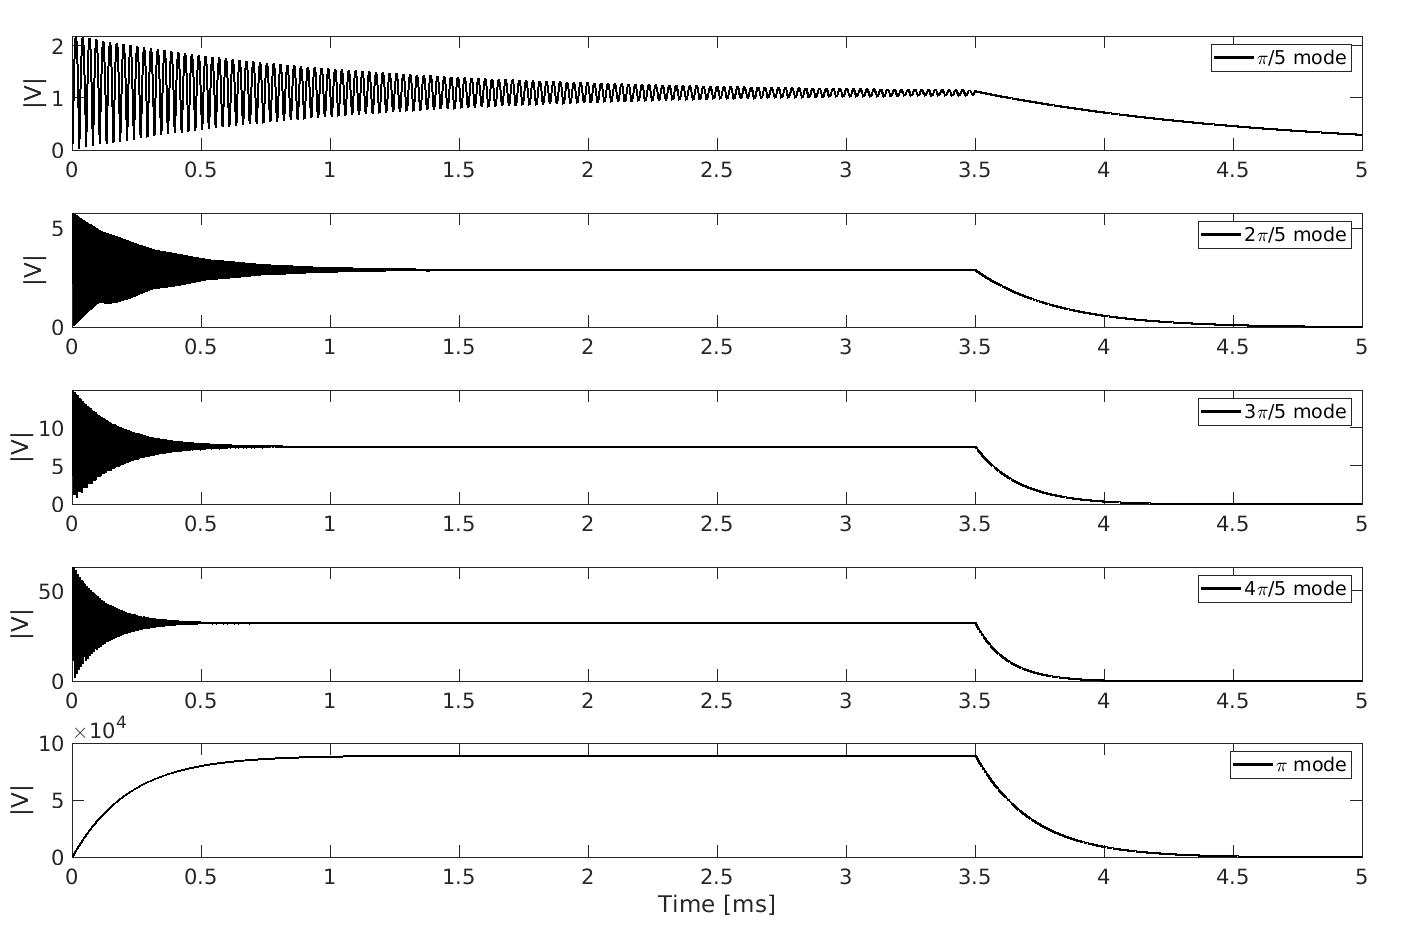
\includegraphics[width=0.65\textwidth]{./09-mode-amplitudes.png}
  \caption{\label{fig:modamp}模态幅度。请注意五幅图的纵轴尺度范围很大。下方图中的 $\pi$ 模幅度远大于另外四幅图。} 
\end{center}
\end{figure}
% ..............................................
从紧跟方程~\ref{eq:c1t}之后的讨论来看，人们可能会以为腔体的填充时间 $\tau$ 由 $1/\tau=\ho_1/2Q'_L$ 给出。然而，实际上它由对应腔体 $\pi$ 模激发的本征值实部决定。为了进一步研究这一点，我们在图~\ref{fig:eigval}中展示了 10 个本征值。上图显示本征值的实部，下图显示对应的虚部，而虚部要比相应的实部大得多。我们还注意到，本征值成复共轭对出现；相邻实部的大小相同，而对应的虚部符号相反。这里较大的虚部表明该模主要表现为振荡。它们负责脉冲开始时腔体电压的振荡行为，这在图~\ref{fig:fivea}中已经突出显示。本征值 1 和 2 的实部特别小，因此对应模态的振荡会持续相当长的时间。与此同时，它们的虚部很大，因此振荡也非常明显。这解释了图~\ref{fig:fiveb}中虚部，也就是 Q 相位的激发。前八个本征值之所以会被激发，是因为发生器脉冲的突升包含许多频率，其中有些频率落在前四个模态的带宽内，而这些模态由前八个本征值描述。另一方面，编号 9 和 10 的本征值对具有最小的虚部（红色），同时仍保持适中的实部（蓝色）。因此，这两个模态主要吸收发生器提供的能量。
\par
图~\ref{fig:eigvec}上排显示的是奇数编号的本征矢。实部用蓝色表示，虚部用红色表示。它们之所以按五个一组出现，是因为把复值方程~\ref{eq:dynp}转换为其实值对应式~\ref{eq:dynpb}时，对电压进行了重新排序。我们看到，模态图样与图~\ref{fig:evs}中已经出现的模态一致。只是在这里，实部（蓝色）和虚部（红色）彼此对应。下排显示的是复共轭的偶数编号本征矢。它们的实部（蓝色）与上面对应图相同，但虚部（红色）的符号相反。
\par
特别地，本征矢 9 和 10 展示了 $\pi$ 模的激发图样，相邻单元具有相反极性。值得注意的是，我们已经发现对应本征值 9 和 10 的虚部特别小，因此该模态并不以振荡为主，而是吸收了发生器提供的大部分能量。并且，本征值的实部决定了 $\pi$ 模的填充时间 $\tau=1/\real(\lambda_9)$。将其数值与 $1/\tau'= \ho/2Q'_L$ 比较可知，$\tau=5\tau'$。填充五单元腔比填充单个单元要多花五倍时间。毕竟，我们必须提供功率去填满五个单元，而不是一个，这自然会多花五倍时间。换一个角度看：这五个单元就像五个串联的带通滤波器，因此整体带宽缩小了五倍。
\par
为了观察五个模态的时间依赖性，我们构造它们各自本征子空间上的投影算符。这些本征子空间由 $W$ 的列张成，而这些列就是方程~\ref{eq:WLW}中矩阵 $W$ 的本征矢。因此我们可以写成
\begin{equation}
W=\left(\ket{w_1},\ket{w_2},\dots,\ket{w_{10}}\right)\ .
\end{equation}
这里我们借用量子力学中的 bra 和 ket 记号，其中 ket 表示列向量，即矩阵 $W$ 的列本征矢 $\ket{w_i}$，$i=1,\dots,10$。类似地，我们把 $W^{-1}$ 的行向量记为 $\bra{w_i}$，因此
\begin{equation}
W^{-1}=\left(\begin{array}{c}\bra{w_1}\\ \vdots \\ \bra{w_{10}}\end{array}\right)\ .
\end{equation}
利用这一记号，我们可以把方程~\ref{eq:WLW}改写为谱分解形式
\begin{equation}
  \tilde A =\sum_{i=1}^{10}\lambda_i P_i
  \qquad\mathrm{with}\qquad
  P_i=\ket{w_i}\bra{w_i}\ ,
\end{equation}
其中 $P_i$ 是投影到由本征值 $\lambda_i$ 所表征的子空间上的投影算符，而 $\ket{w_i}\bra{w_i}$ 是列向量 $\ket{w_i}$ 与行向量 $\bra{w_i}$ 的外积。注意 $\tilde A$ 不是对称矩阵，因此 $W$ 既不是实矩阵，也不是正交矩阵。由于本征值成复共轭对出现，例如我们用 $P_1$ 和 $P_2$ 的和，即 $Q_1=P_1+P_2$，来确定 $\pi/5$ 模对电压 $\tilde V(s)$ 的贡献，记为 $V(\pi/5)=Q_1\tilde V(s)$。其他模态的投影算符构造方式类似。图~\ref{fig:modamp}上图显示了该模态的幅度，即 $V(\pi/5)$ 的范数。我们看到它只缓慢衰减，这是因为本征值 $\lambda_1$ 和 $\lambda_2$ 的实部最小，因此对应最长的时间常数，正如前面所讨论的那样。除了下图中显示的 $\pi$ 模之外，所有模态在发生器于 3.5\,ms 关闭之前就已经衰减到很小的值。只有 $\pi$ 模的幅度增长到远大于其他四个模态的程度，并且表现出与图~\ref{fig:fiveb}和~\ref{fig:fivec}上图相同的行为。
\par
%..............................................
\begin{figure}[b]
\begin{center}
  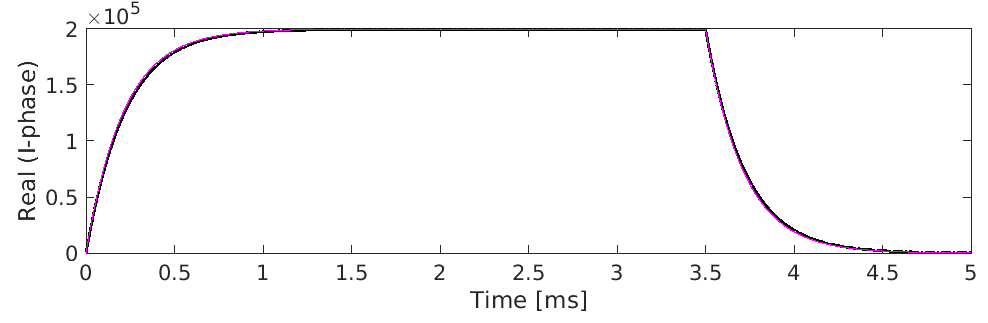
\includegraphics[width=0.8\textwidth]{./19-five-single-cell-comparison_upper.png}
  \caption{\label{fig:comp}单单元腔中的电压（品红）叠加在五单元腔中的电压（黑色）之上。} 
\end{center}
\end{figure}
% ..............................................
把以 $\pi$ 模运行的五单元腔与单单元腔进行比较是很有启发性的。在没有任何缺陷的情况下，我们用~\cite{VZAP}描述由电流 $I$ 驱动的单单元谐振器中的电压 $V$
\begin{equation}
  \frac{dV}{dt}=-\oo V +\frac{\oo R}{1+\beta} I
  \qquad\mathrm{with}\qquad
  \oo=\frac{\ho}{2 Q_L}=(1+\beta)\frac{\ho}{2Q}\ .
\end{equation}
该方程很容易积分，因此在开启发生器之后的电压为
\begin{equation}
  V(t) = \left( 1-e^{-\oo t}\right) V_{\infty}
  \qquad\mathrm{with}\qquad
  V_{\infty}=\frac{IR}{1+\beta}\ ,
\end{equation}
其中 $V_{\infty}$ 是渐近稳态电压。发生器关闭后，电压按指数形式衰减 $V(t)=V_ae^{-\oo t}$，其中 $V_a$ 是发生器关闭前一瞬间的电压。
\par
图~\ref{fig:comp}显示的是单单元腔的电压叠加在以 $\pi$ 模运行的五单元腔第 1、3、5 单元的电压之上。后者已经在图~\ref{fig:fiveb}的上图中给出。在单单元模型中，我们必须把 $Q$、也就是时间常数 $1/\oo$，提高五倍，以对应于填充五个单元而不是一个单元。但这样一来，图~\ref{fig:comp}中的曲线几乎完全一致，从而在很大程度上证明了用单单元等效模型近似多单元腔这一常见做法是合理的。
\par
在讨论完美的 $\pi$ 模腔之后，我们现在转向各种缺陷带来的后果，例如单元间耦合 $\kappa_i$ 不正确，或者某个单元的本征 $Q$ 值 $Q_i$ 和谐振频率 $\ho_i$ 偏离设计值。
%
\section{单元间耦合误差 $\kappa_i$}
\label{sec:kappa}
%
现在我们假设各个 $\kappa_i$ 可能与其设计值 $\kappa$ 相差 $\Dk_i$。我们还假设所有电容 $C_i$ 都相等，因此有 $\kappa'_j=\kappa_{j-1}$。此外，与束流管的耦合也可以偏离设计值，满足 $\kappa_a=2\kappa+\Delta\kappa_a$ 和 $\kappa_b=2\kappa+\Delta\kappa_b$。这就迫使我们把第一个单元的方程~\ref{eq:c1t} 和~\ref{eq:c1tp}修改为
\begin{eqnarray}\label{eq:c1tk}
  &&\left(2+6\kappa+\kappa_1+\Dk_a\right)\frac{d\tV_1}{dt} -\kappa_1\frac{d\tV_2}{dt}\\
  &&\qquad=-\frac{\ho}{Q'_L}\tV_1
         +i\frac{\ho}{\sqrt{1+4\kappa}}\left[(2\kappa-\kappa_1-\Dk_a)\tV_1+\kappa_1\tV_2\right]
         + \frac{\ho R_1}{Q_1}\frac{\tilde I_g}{n}\ .\nonumber
\end{eqnarray}
对于腔体中间的单元，方程~\ref{eq:cjt} 和~\ref{eq:cjtp}修改为
\begin{eqnarray}\label{eq:cjtk}
  &&-\kappa_{j-1} \frac{d\tV_{j-1}}{dt}
     +\left(2+4\kappa+\kappa_{j-1}+\kappa_j\right)\frac{d\tV_j}{dt}
  -\kappa_j \frac{d\tV_{j+1}}{dt}\\
   &&\qquad\quad = -\frac{\ho}{Q}\tV_j+\frac{i\ho}{\sqrt{1+4\kappa}}\left[\kappa_{j-1}\tV_{j-1}
      +\left(4\kappa-\kappa_{j-1}-\kappa_j\right)\tV_j+\kappa_j\tV_{j+1} \right]\ .\nonumber
\end{eqnarray}
最后，描述最后一个单元~$n$ 的方程~\ref{eq:cnt} 和~\ref{eq:cntp}变为
\begin{eqnarray}\label{eq:cntk}
  &&-\kappa_{n-1} \frac{d\tV_{n-1}}{dt}
  +\left(2+6\kappa+\kappa_{n-1}+\Dk_b\right)\frac{d\tV_j}{dt} \\
   &&\qquad\qquad = -\frac{\ho}{Q}\tV_n +\frac{i\ho}{\sqrt{1+4\kappa}}\left[\kappa_{n-1}\tV_{n-1}
      +\left(2\kappa-\kappa_{n-1}-\Dk_b\right)\tV_n\right]\ .\nonumber
\end{eqnarray}
在仿真中，我们把这些方程转换为矩阵形式。与方程~\ref{eq:dynpaux}相比，只需要把矩阵 $D$ 和 $B$ 修改为
%\scriptsize{  
{\tiny
\begin{eqnarray}
  D&=&\left(\begin{array}{ccccc}
     2+6\kappa+\kappa_1+\Dk_a & -\kappa_1 & 0 & 0 & 0 \\
     -\kappa_1 & 2+4\kappa+\kappa_1+\kappa_2 & -\kappa_2 & 0 & 0 \\
     0 & -\kappa_2 & 2+4\kappa+\kappa_2+\kappa_3 & - \kappa_3 & 0 \\
     0 & 0 & -\kappa_3 & 2+4\kappa+\kappa_3+\kappa_4 & - \kappa_4 \\
     0 & 0 &  0 &-\kappa_4 & 2+6\kappa+\kappa_4+\Dk_b
   \end{array}\right)\nonumber\\
  B&=&\frac{\ho\dt}{\sqrt{1+4\kappa}}\left(\begin{array}{ccccc}
              2\kappa-\kappa_1-\Dk_a & \kappa_1 & 0 & 0 & 0\\
              \kappa_1 & 4\kappa-\kappa_1-\kappa_2 & \kappa_2 & 0 & 0\\
              0 & \kappa_2 & 4\kappa-\kappa_2-\kappa_3 & \kappa_3 & 0\\
              0 & 0 & \kappa_3 & 4\kappa-\kappa_3-\kappa_4 & \kappa_4\\
              0 & 0 & 0 & \kappa_4 & 2\kappa-\kappa_4-\Dk_b
       \end{array}\right)\ .
\end{eqnarray} }% end of tiny
很容易看出，如果所有 $\kappa_i$ 都等于 $\kappa$，并且 $\Dk_a$ 和 $\Dk_b$ 都为零，这些表达式就会回到方程~\ref{eq:dynpaux}中的形式。
\par
%..............................................
\begin{figure}[tb]
\begin{center}
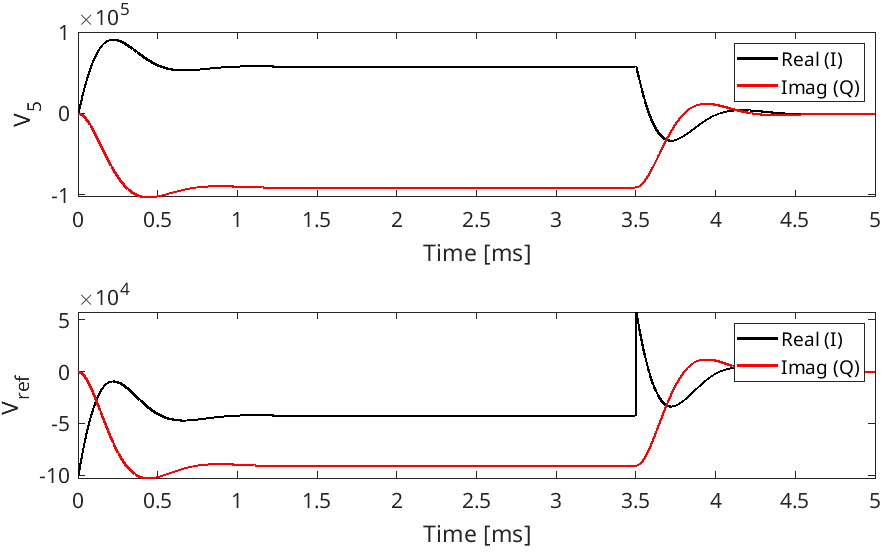
\includegraphics[width=0.57\textwidth]{./11-five-5ms-fwd-ref-dk2.png}
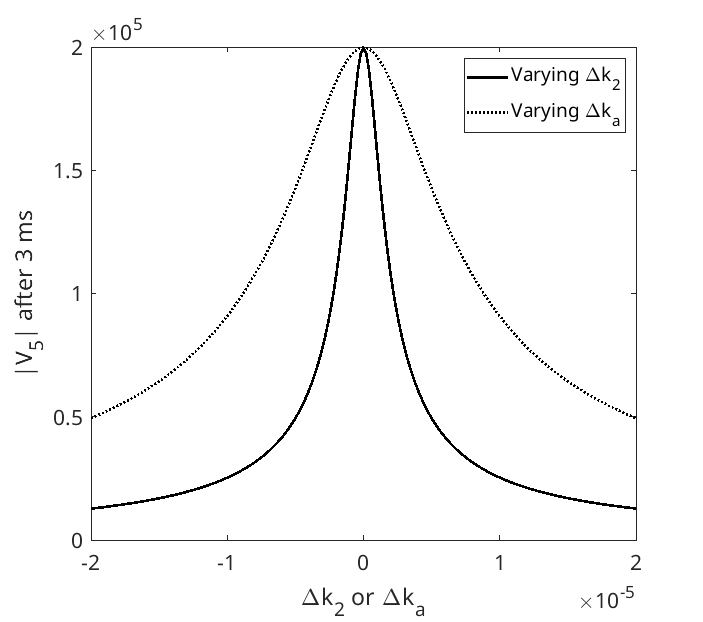
\includegraphics[width=0.4\textwidth]{./12-resonance-k2.png}
\end{center}
\caption{\label{fig:fivedk2}左图对应图~\ref{fig:fivec}，不过这里第二和第三单元之间的耦合相对于设计值 $\kappa_2=0.01$ 增加了 $\Dk_2=2\times 10^{-6}$。右图显示的是 3\,ms 后第 5 单元电压幅度 $|V_5|$ 随 $\Dk_2$（实线）和 $\Dk_a$（虚线）的变化，范围为 $\pm2\times 10^{-5}$。}
\end{figure}
% ..............................................
图~\ref{fig:fivedk2}左图上半部分显示第 5 单元场的 I 相和 Q 相，下半部分显示反射信号。这里第二和第三单元之间的耦合相对于图~\ref{fig:fivec}中的情况增加了 $\Dk_2=2\times10^{-6}$。在上图中我们看到，与图~\ref{fig:fivec}相比，最大可达到的信号从 $2\times 10^5$ 明显降到了 $1.3\times 10^5$，而且在上下两个图中都出现了明显的虚部，也就是 Q 相（红色）。此外，信号中还能看到一定的振铃。结果表明，在图~\ref{fig:fivec}所示情况下纯实的 $\pi$ 模本征值现在获得了一个很小的虚部，从而引发了振荡的出现。若进一步增大 $\Dk_2$，振铃会变得非常明显，不过我们这里不再给出图示。
\par
图~\ref{fig:fivedk2}右图中的实线显示第 5 单元场幅度 $|V_5|$ 随 $\Dk_2$ 的变化，呈现出明显的类共振行为。该曲线的半高全宽为 $4.2\times 10^{-6}$，这可以作为制造腔体、尤其是单元间耦合的公差指标。虚线显示的是在相同范围内改变与束流管耦合 $\kappa_a$ 的响应 $\Dk_a$。我们发现这条曲线大约宽三倍，说明腔体两端的制造公差可以稍微放宽一些。
\par
下一节我们将对单元本征品质因数 $Q_i$ 的变化做类似分析。
% 
\section{单元品质因数 $Q_i$ 误差}
\label{sec:Q}
%..............................................
\begin{figure}[tb]
\begin{center}
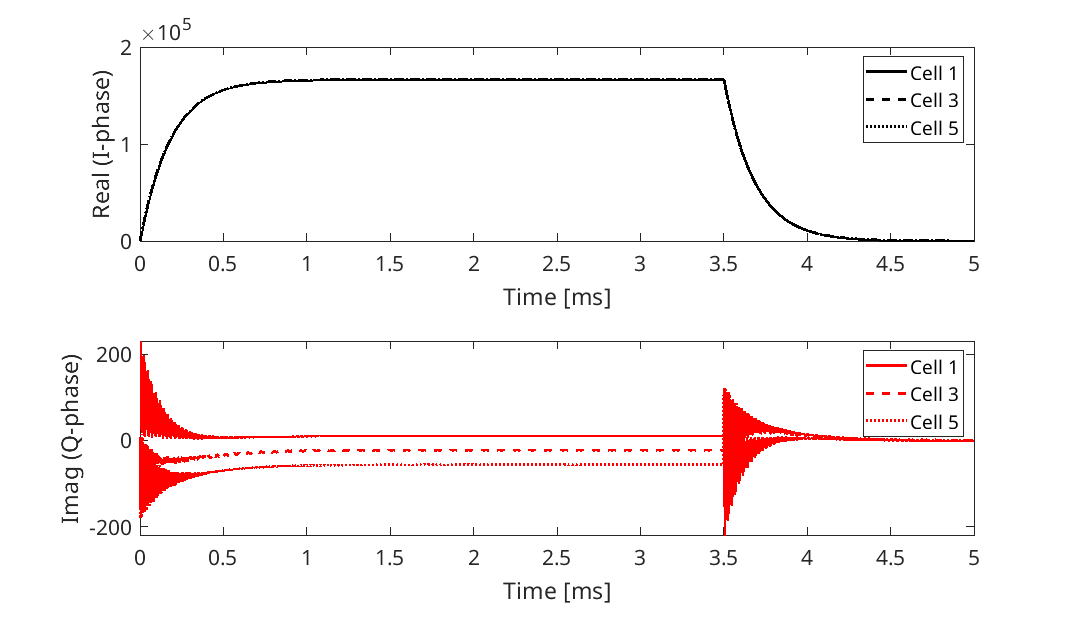
\includegraphics[width=0.6\textwidth]{./13-five-cell135-Q.png}
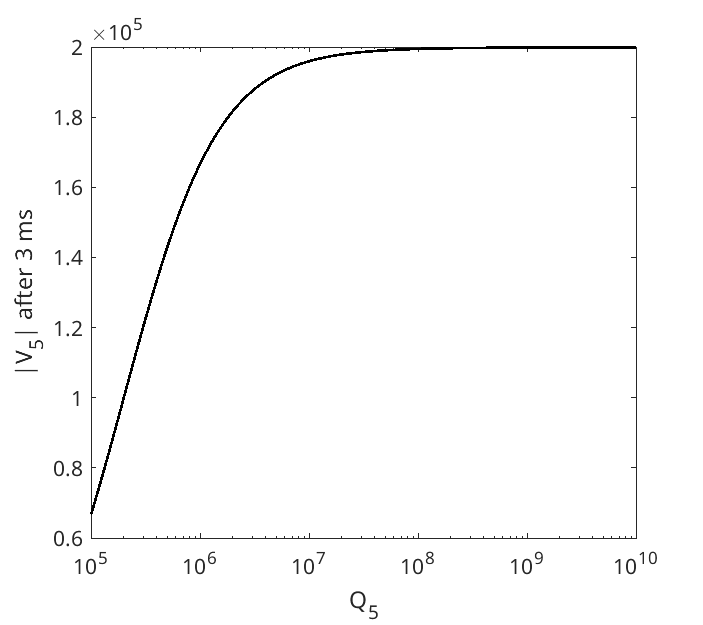
\includegraphics[width=0.38\textwidth]{./13-five-resonance-Q.png}
\end{center}
\caption{\label{fig:fiveQ}左图对应图~\ref{fig:fiveb}，只不过这里第 5 单元的品质因数 $Q_5$ 被降低了 1000 倍，变为 $10^6$。右图显示第 5 单元电压幅度 $|V_5|$ 在 3\,ms 后随 $Q_5$ 的变化，范围为 $10^5$ 到 $10^{10}$。}
\end{figure}
% ..............................................
单元中的损耗通过改变单元电阻 $R_i$ 来建模，这主要影响品质因数 $Q_i=R_i\sqrt{C_i/L_i}$，同时也影响第 1 单元的耦合 $\beta=R_1/n^2Z_0$。为了考虑这些损耗，我们只需把方程~\ref{eq:dynpaux}中的数组 $A$ 修改为
\begin{equation}
  A=\diag\left((1+\beta)\frac{\ho\dt}{Q_1}, \frac{\ho\dt}{Q_2}, \frac{\ho\dt}{Q_3},
    \frac{\ho\dt}{Q_4},\frac{\ho\dt}{Q_5}\right)
\end{equation}
其余量保持不变。图~\ref{fig:fiveQ}左图对应图~\ref{fig:fiveb}，后者显示的是未受扰动的系统。这些图展示了脉冲过程中第 1、3 和 5 单元电压的 I 相和 Q 相。只不过这里第 5 单元的品质因数 $Q_5$ 从 $10^9$ 降低了 1000 倍，变为 $10^6$。上图显示的是电压的实部，也就是 I 相。与图~\ref{fig:fiveb}相比，我们观察到幅度略有减小。$Q_5$ 的降低使下图中的虚部，也就是 Q 相，在三个单元之间出现了轻微分裂。我们将其解释为第 5 单元吸收了穿过前面单元的大部分功率，而且损耗略大于发生器能够持续补充的能量。
\par
图~\ref{fig:fiveQ}右图显示第 5 单元电压绝对值 $|V_5|$ 随 $Q_5$ 的变化。只要只有 $Q_5$ 被降低，而且耗散能量不会使相邻单元淬灭，电压 $|V_5|$ 受到的影响就很小，除非它降到几倍 $10^6$ 以下。
\par
%..............................................
\begin{figure}[tb]
\begin{center}
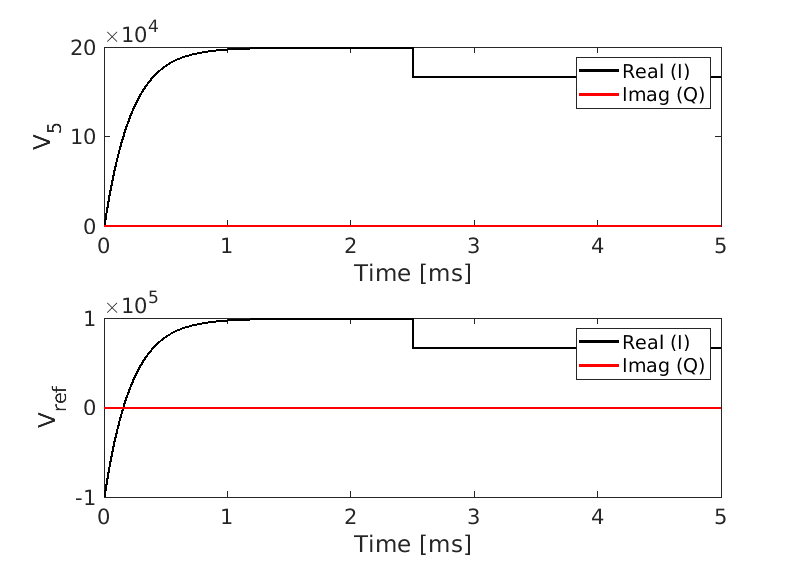
\includegraphics[width=0.47\textwidth]{./17-five-cell1_quench_x1e3.png}
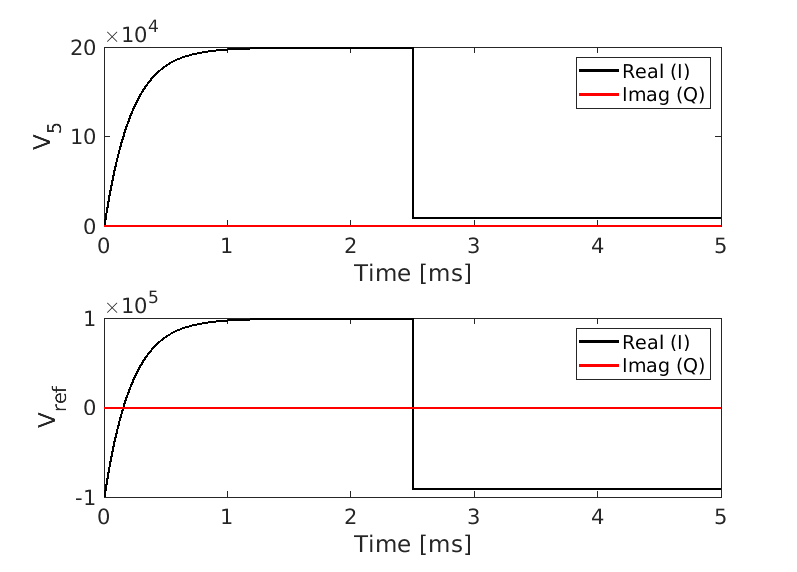
\includegraphics[width=0.47\textwidth]{./17-five-cell1_quench_x1e5.png}
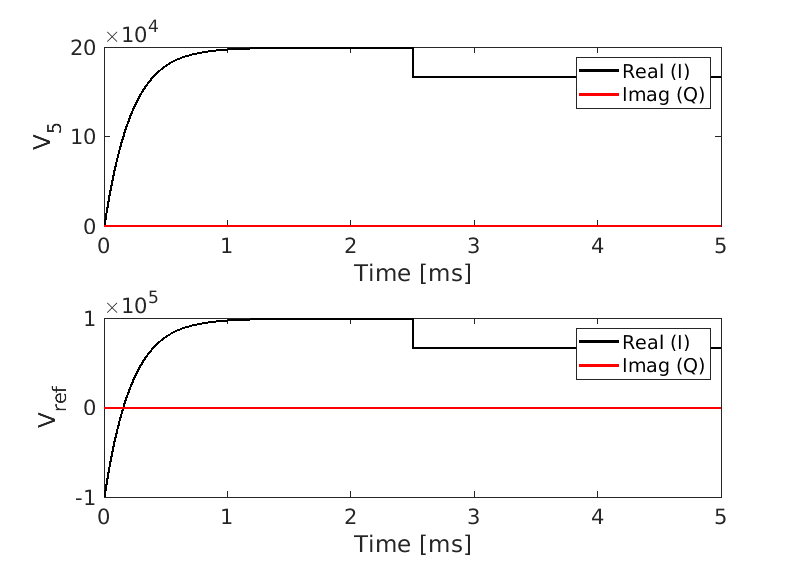
\includegraphics[width=0.47\textwidth]{./18-five-cell4_quench_x1e3.png}
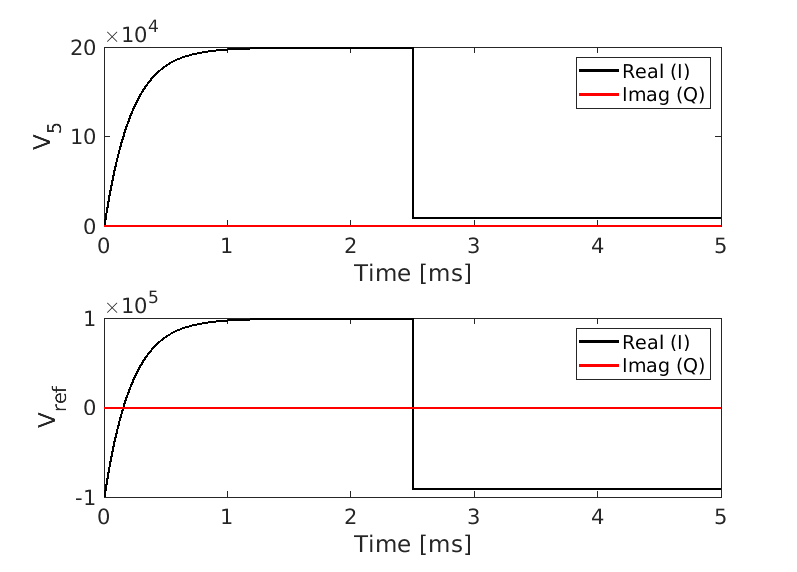
\includegraphics[width=0.47\textwidth]{./18-five-cell4_quench_x1e5.png}
\end{center}
\caption{\label{fig:quench}第 5 单元电场 $V_5$ 和反射信号 $V_{ref}$，对应第 1 单元在 2.5\,ms 后发生淬灭的情形。左图中电阻 $R_1$ 下降 $x=10^3$，右图中下降 $10^5$。}
\end{figure}
%..............................................
第 1 单元损耗的增加需要稍加注意，因为 $Q_1$ 和 $\beta$ 都会受到影响。设电阻 $R_1$ 下降某个因子 $x$。较大的淬灭对应较大的 $x$，比如 $10^5$。这个因子会把 $Q_1$ 降到 $Q_1/x$，并把 $\beta$ 降到 $\beta/x$，因此矩阵 $A$ 的第一项会变成 $(1+\beta/x)/(Q_1/x)=(x+\beta)/Q_1$，其中 $Q_1$ 和 $\beta$ 是默认值。这里可以看出，只要 $x$ 小于 $\beta$，第 1 单元的淬灭对矩阵 $A$ 第一项所对应的时间常数只会有温和影响。
\par
图~\ref{fig:quench}中的每幅图都显示第 5 单元场 $V_5$ 和反射信号 $V_{ref}$，对应在 2.5\,ms 后发生淬灭的情况。上排图中第 1 单元发生淬灭。我们通过把电阻 $R_1$ 分别降低 $x=10^3$（左）和 $x=10^5$（右）来模拟。较弱的淬灭，如左图所示，只会让电压 $V_5$ 有适度下降；而较强的淬灭，如右图所示，则会使腔体中的场几乎完全崩溃，并相应改变反射信号。下排两图对应第 4 单元等幅度的淬灭，我们通过降低 $R_4$ 来模拟。我们发现 $V_5$ 和 $V_{ref}$ 的行为与上排图非常相似。
\par
最后，让我们考虑一个或多个单元失谐时会发生什么。
%
\section{单元失谐}
\label{sec:omega}
%
在本节中，我们假设第 $j$ 个单元的谐振频率 $\ho_j$ 与设计值 $\ho$ 的偏差为 $\Do_j=\ho_j-\ho$。此外，对于 $\pi$ 模，我们有 $\ho^2/\omega^2_{\pi}=1+4\kappa$，因此得到
\begin{equation}
  \frac{\ho^2_j}{\omega_{\pi}^2}=\frac{\ho^2+2\ho\Do_j+\Do_j^2}{\omega_{\pi}^2}
  %\approx \frac{\ho^2+2\ho\Do_j}{\omega_{\pi}^2}
  %=1+4\kappa-2\frac{\ho^2}{\omega_{\pi}^2}\frac{\Do_j}{\ho}
  \approx 1+4\kappa+2\frac{\Do_j}{\ho}
  \approx 1+4\kappa + \delta_j
\end{equation}
其中我们用缩写 $\delta_j=2\Do_j/\ho$ 来描述第 $j$ 个单元的相对失谐。
\par
在假设其他参数都等于设计值的情况下，第一个单元的方程变为
\begin{eqnarray}\label{eq:c1td}
&&  \left(2+7\kappa+\delta_1\right)\frac{d\tV_1}{dt} -\kappa\frac{d\tV_2}{dt}\\
&&\qquad\qquad  =-\frac{\ho}{Q'_L}\tV_1
  +i\frac{\ho}{\sqrt{1+4\kappa}}\left[(\kappa+\delta_1)\tV_1+\kappa\tV_2\right]
  + \frac{\ho R_1}{Q_1}\frac{\tilde I_g}{n}\ .\nonumber
\end{eqnarray}
对于腔体中部的第 $j$ 个单元，我们得到
\begin{eqnarray}\label{eq:cjtd}
&&  -\kappa \frac{d\tV_{j-1}}{dt} +\left(2+6\kappa+\delta_j\right)\frac{d\tV_j}{dt}
     -\kappa \frac{d\tV_{j+1}}{dt}\\
  &&\qquad\qquad = -\frac{\ho}{Q}\tV_j+i\frac{\ho}{\sqrt{1+4\kappa}}
     \left[\kappa\tV_{j-1} +(2\kappa+\delta_j)\tV_j+\kappa\tV_{j+1} \right]
     \nonumber
\end{eqnarray}
最后一个单元的方程为
\begin{eqnarray}\label{eq:cntd}
  && -\kappa \frac{d\tV_{n-1}}{dt}+\left(2+7\kappa+\delta_n\right)\frac{d\tV_j}{dt}\\
  &&\qquad\qquad = -\frac{\ho}{Q}\tV_n +i\frac{\ho}{\sqrt{1+4\kappa}}
      \left[\kappa\tV_{n-1}+(\kappa+\delta_n)\tV_n\right]\ .\nonumber
\end{eqnarray}
在所有方程中，我们把 $\ho_j/Q_j$ 近似为 $\ho/Q$，因此忽略了失谐对阻尼的极小影响。这使得仿真中使用的矩阵 $A$ 不受影响。另一方面，单元谐振频率的变化主要影响矩阵 $D$ 和 $B$
\begin{eqnarray}
  D&=&\left(\begin{array}{ccccc}
     2+7\kappa+\delta_1 & -\kappa & 0 & 0 & 0 \\
     -\kappa & 2+6\kappa+\delta_2 & - \kappa & 0 & 0 \\
     0 & -\kappa & 2+6\kappa+\delta_3 & - \kappa & 0 \\
     0 & 0 & -\kappa & 2+6\kappa+\delta_4 & - \kappa \\
     0 & 0 &  0 &-\kappa & 2+7\kappa+\delta_5
   \end{array}\right)\nonumber\\
  B&=&\frac{\ho\dt}{\sqrt{1+4\kappa}}\left(\begin{array}{ccccc}
       \kappa+\delta_1& \kappa & 0 & 0 & 0\\
              \kappa & 2\kappa+\delta_2 & \kappa & 0 & 0\\
              0 & \kappa & 2\kappa+\delta_3 & \kappa & 0\\
              0 & 0 & \kappa & 2\kappa+\delta_4 & \kappa\\
              0 & 0 & 0 & \kappa & \kappa+\delta_5
 \end{array}\right)\ 
\end{eqnarray}
这就使得在仿真中纳入失谐单元变得很直接。
\par
%..............................................
\begin{figure}[tb]
\begin{center}
  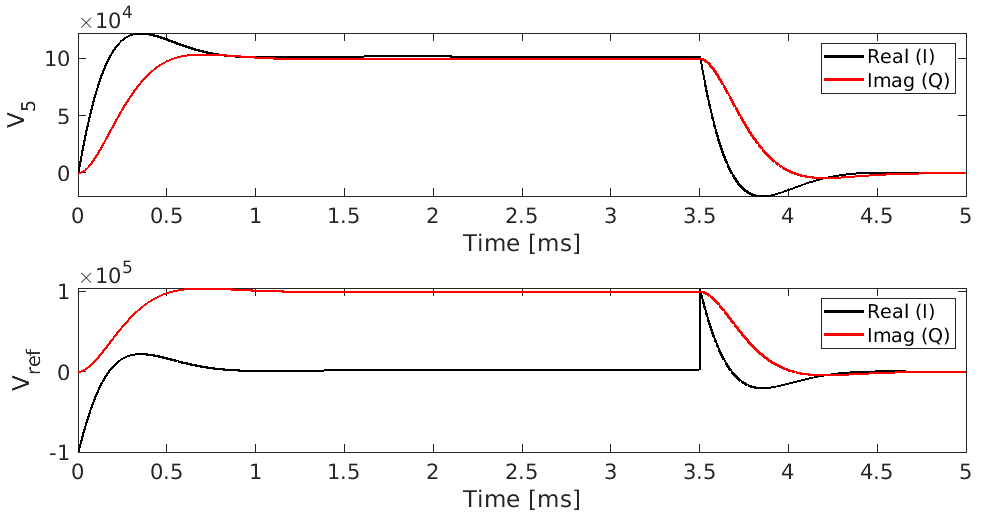
\includegraphics[width=0.65 \textwidth]{./15-five-cell4_detuned_5e-6.png}
  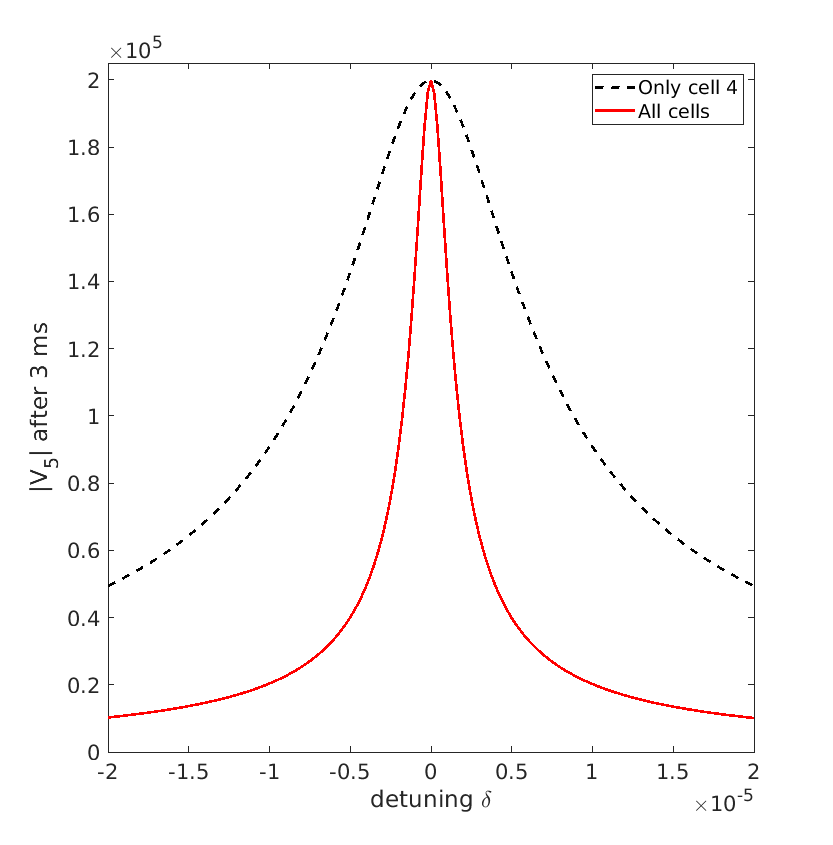
\includegraphics[width=0.34\textwidth]{./15-five-resonance-detuning.png}
\end{center}
\caption{\label{fig:fivedetuning}该图对应图~\ref{fig:fiveQ}，不过左图中第 4 单元失谐 $\delta_4=5\times 10^{-6}$。右图显示第 5 单元电压幅度 $|V_5|$ 随第 4 单元失谐 $\delta$（黑色虚线）以及所有单元以相同量失谐（红色）的变化。}
\end{figure}
% ..............................................
在本节的仿真中，我们保持所有参数为默认值，只改变失谐量。图~\ref{fig:fivedetuning}左图上半部分显示第 5 单元电压 $V_5$，下半部分显示反射信号 $V_{ref}$。在该仿真中，第 4 单元失谐 $\delta_4=5\times10^{-6}$，这大致对应腔体加载带宽 $(1+\beta)/2Q$ 的两倍。我们看到，$V_5$ 和 $V_{ref}$ 的实部与虚部具有相近的幅度，这表明失谐的影响相当明显。我们还观察到 $V_5$ 的幅度减小。顺便提一下，如果让所有单元都失谐 $\delta=10^{-6}$，也就是 $\delta_4$ 的五分之一，那么 $V_5$ 和 $V_{ref}$ 的图几乎不变。换句话说，仅从观测透射信号 $V_5$ 和反射信号 $V_{ref}$，我们无法判断是一个单元失谐还是所有单元都以更小的量失谐。最后，图~\ref{fig:fivedetuning}右图显示第 5 单元幅度 $|V_5|$ 随失谐量的变化。黑色虚线对应第 4 单元失谐，红色曲线对应所有单元以相同失谐量 $\delta$ 失谐。我们看到红色曲线比黑色曲线窄得多，这表明与只让单个单元失谐相比，让所有单元都失谐时的敏感性高得多。
%
\section{结论}
%
我们发现，多单元腔的行为与单单元腔非常相似，这从图~\ref{fig:comp}中两条曲线的高度一致性可以看出。原因在于 $\pi$ 模只需大约微秒量级就能形成，如图~\ref{fig:fivea}所示。其他模态虽然被激发，但它们并不会吸收功率来建立一个相干模态。相反，它们会逐渐衰减，如图~\ref{fig:modamp}上方四幅图所示，其中各自的时间常数与图~\ref{fig:eigval}中本征值的实部相关。基本上，除了其他模态短暂的瞬态之外，$\pi$ 模主导了多单元腔中电磁场的动力学，并作为一个整体振荡，而不是让单元中弱耦合的场各自独立振荡。
\par
$\pi$ 模作为一个整体振荡这一事实会影响单元制造公差，因为 $\pi$ 模会对各个缺陷的贡献进行平均。我们确定了对单元间耦合 $\kappa$ 的公差，并将结果显示在图~\ref{fig:fivedk2}右图中，该图给出了一条类共振曲线，其宽度决定了对 $\kappa$ 的敏感性。此外，图~\ref{fig:fivedetuning}右图显示了对单元失谐的敏感性，这比所有单元以相同量失谐要宽松得多。在图~\ref{fig:quench}中，我们发现如果某个单元的淬灭在“较小”的意义上成立，也就是其损耗与通过输入耦合器逸出的损耗相当，那么单元中的淬灭可以被稳定下来，这由 $\beta$ 给出。如果某个单元的降低因子 $x=Q/Q_{quench}\gg\beta$，那么淬灭会导致 $\pi$ 模崩溃，如图~\ref{fig:quench}右图所示。
\par
% Unfortunately, we could not find signals in the transmitted $V_5$ and
% reflected $V_{ref}$ signal can allow to infer which cell is causing the
% observed signal. Also this is a consequence that the $\pi$-mode ``averages''
% over the entire cavity~\cite{SLATER}.
% \par
本报告中开发的方法可以很容易地推广到其他腔体，并可用于估计多种缺陷的制造公差，例如 $Q$ 值的均匀性，或者统计分布的耦合 $\kappa$ 或失谐 $\delta=2\Do/\ho$。
\par
特别值得关注的是图~\ref{fig:fivea}中显示的初始高频振荡。用高速数据采集系统对其进行实验测量，并用用于测量 $Q_0$ 的方法~\cite{Q0}从理论上确定它们与腔体缺陷之间的关系，似乎是一项值得开展的工作。
\par
本工作部分由 Jefferson Science Associates, LLC 在美国能源部合同号 AC05-06OR23177 下完成。出版方承认美国政府享有许可权，并根据 DOE 公共获取计划（\url{http://energy.gov/downloads/doe-public-access-plan}）提供公开访问。
%
%%%%%%%%%%%%%%%%%%%%%%%%%%%%%%%%%%%%%%%%%%%%%%%%%%%%%%%%%%%%%%%%%%%%%%%
%
\bibliographystyle{plain}
\begin{thebibliography}{M}
  %
\bibitem{SCHILCHER}
  T. Schilcher, {\em 洛伦兹力失谐超导腔中脉冲加速场的矢量和控制，} 博士论文，Universit\"at Hamburg，1998.
\bibitem{SYSID}
  V. Ziemann, {\em 使用递归最小二乘算法对超导腔实时系统辨识的仿真，} Physical Review Accelerators and Beams 26 (2023)
  112003.
\bibitem{PKH}
  H. Padamsee, J. Knobloch, T. Hays, {\em 面向加速器的射频超导技术，第 2 版，}
  Wiley-VCH, Weinheim, 2008.
\bibitem{LIEPE}
  M. Liepe, {\em 用于直线对撞机的超导多单元腔，} 博士论文，
  Universit\"at Hamburg, 2001.
\bibitem{PLASMA}
  T. Powers, N. Brock, T. Ganey {\em JLab 超导腔原位等离子体处理：2023 更新，} 第 21 届射频超导国际会议 SRF2023 论文集 (2023) 701.
\bibitem{VZAP}
  V. Ziemann, {\em 使用 MATLAB 的加速器物理实战，第 2 版，}
  CRC Press, Boca Raton, 2025.
\bibitem{Q0}
  V. Ziemann, {\em 测量超导腔本征品质因数的一种新方法，}
  Physical Review Accelerators and Beams 27 (2024) 032001;
% \bibitem{SLATER}
%   J.C. Slater, {\em Microwave Electronics,} D. Van Nostrand Company, Inc., 1950.
%\bibitem{ABRASTE}
% M. Abramowitz, I. Stegun, {\em Handbook of Mathematical Functions,}
% Dover, New York, 1972.
%
\end{thebibliography}
%
\end{document}
